% Guida del relatore — ZISAR, seminario GSSI 30 ottobre 2026
% Compile: tectonic guida_relatore.tex
\documentclass[11pt,a4paper]{article}
\usepackage[T1]{fontenc}
\usepackage[italian]{babel}
\usepackage{mathpazo}
\usepackage{amsmath,amssymb,bm,mathtools}
\usepackage[margin=2.3cm]{geometry}
\usepackage{booktabs,multirow,array}
\usepackage{parskip}
\usepackage{enumitem}
\usepackage{xcolor}
\usepackage[colorlinks=true,linkcolor=blue!60!black,citecolor=blue,urlcolor=blue]{hyperref}
\usepackage{tcolorbox}
\usepackage{etoolbox}

\definecolor{navy}{RGB}{24,52,97}
\definecolor{accent}{RGB}{213,94,0}
\newtcolorbox{warn}{colback=accent!6,colframe=accent,boxrule=0.6pt,arc=2pt,left=4pt,right=4pt,top=3pt,bottom=3pt,title=\textbf{Possibile challenge},fonttitle=\small}
\newtcolorbox{say}{colback=navy!5,colframe=navy,boxrule=0.6pt,arc=2pt,left=4pt,right=4pt,top=3pt,bottom=3pt}
\newcommand{\app}[1]{{\small\color{navy}[$\to$ App.~\ref{#1}]}}
% Schede per imparare il talk. \scheda[ponte se salti la prossima]{pagina}{titolo}{messaggio}{numeri}{ponte}
% stampa il riquadro sotto la slide e aggiunge la riga alla scaletta e alla lista dei titoli
% (parte ``Schede per le prove''); \schedasez{pagina}{sezione}{minuti}{gancio}{ponte} fa lo stesso per le slide di sezione.
\newtcolorbox{schedabox}{colback=navy!4,colframe=navy!60,boxrule=0.5pt,arc=2pt,left=4pt,right=4pt,top=2pt,bottom=2pt,fontupper=\small}
\newcommand{\scalettalista}{}\newcommand{\titolilista}{}
\newcommand{\salta}[1]{\ifstrempty{#1}{}{\par{\color{gray}se salti la prossima:} \emph{``#1''}}}
\newcommand{\scheda}[6][]{%
  \begin{schedabox}\textbf{Messaggio.} #4\ifstrempty{#5}{}{\par\textbf{Numeri.} #5}\par
    $\to$\ \textbf{Ponte:} \emph{``#6''}\salta{#1}\end{schedabox}%
  \gappto\scalettalista{\item[#2] \textbf{#3}\par #4\ifstrempty{#5}{}{\par{\color{gray}#5}}\par$\to$\ \emph{``#6''}\salta{#1}}%
  \gappto\titolilista{\item[#2] #3}}
\newcommand{\schedasez}[5]{%
  \begin{schedabox}\textbf{Gancio:} \emph{``#4''}\par$\to$\ \textbf{Ponte:} \emph{``#5''}\end{schedabox}%
  \gappto\scalettalista{\item[#1] \textbf{\color{navy}#2} {\color{gray}(#3)}\par\emph{``#4''}\par$\to$\ \emph{``#5''}}%
  \gappto\titolilista{\item[#1] \textbf{\color{navy}#2} {\color{gray}(#3)}}}
\newcommand{\testoapertura}{\textbf{[pag.~1]} Thank you for having me. I'm Niccolò Salvini, from the Università Cattolica in Rome, and this is joint work with Vincenzo Nardelli.\par
\textbf{[sempre sul titolo]} Before the model, a word about why I am here. This seminar is part of the AISRe post-doctoral scholarship named after Roberto Camagni. Milieu, territorial capital, city networks: much of the vocabulary that regional science uses today without a second thought came from him. A scholarship that sends young researchers to work abroad is a good way to remember someone who built so much of this community. So: thank you to AISRe, and thank you to GSSI for having me.}
\newcommand{\testochiusura}{\textbf{[pag.~39, dopo i quattro punti]} If you take one thing home: zeros and space are not two problems you can fix one at a time. Ignore the zeros and you get space wrong; ignore space and you get the covariates wrong. ZISAR puts both in one likelihood, and it fits in about a second. Thank you.}
\usepackage{graphicx}
\setlength{\fboxsep}{0pt}\setlength{\fboxrule}{0.4pt}
% \slideimg[width]{page}: one slide page of zisar_workshop.pdf, framed, with its label
\newcommand{\slideimg}[2][0.68]{\par\medskip\noindent\begin{center}\fcolorbox{gray}{white}{\includegraphics[width=#1\textwidth,page=#2]{zisar_workshop.pdf}}\\[1pt]{\scriptsize\color{gray}pagina #2 del PDF delle slide}\end{center}\nopagebreak}
\newcommand{\slidequad}[4]{\par\medskip\noindent\begin{center}\begin{minipage}{\textwidth}\centering
\fcolorbox{gray}{white}{\includegraphics[width=0.47\textwidth,page=#1]{zisar_workshop.pdf}}\hfill
\fcolorbox{gray}{white}{\includegraphics[width=0.47\textwidth,page=#2]{zisar_workshop.pdf}}\\[3pt]
\fcolorbox{gray}{white}{\includegraphics[width=0.47\textwidth,page=#3]{zisar_workshop.pdf}}\hfill
\fcolorbox{gray}{white}{\includegraphics[width=0.47\textwidth,page=#4]{zisar_workshop.pdf}}\\[1pt]
{\scriptsize\color{gray}pagine #1--#4 del PDF delle slide}\end{minipage}\end{center}\nopagebreak}

\newcommand{\E}{\mathbb{E}}
\newcommand{\bW}{\mathbf{W}}\newcommand{\bX}{\mathbf{X}}\newcommand{\bZ}{\mathbf{Z}}\newcommand{\by}{\mathbf{y}}
\newcommand{\bu}{\mathbf{u}}\newcommand{\bI}{\mathbf{I}}\newcommand{\bS}{\mathbf{S}}\newcommand{\bH}{\mathbf{H}}
\newcommand{\beeta}{\boldsymbol{\eta}}\newcommand{\bbeta}{\boldsymbol{\beta}}\newcommand{\bgamma}{\boldsymbol{\gamma}}
\newcommand{\btheta}{\boldsymbol{\theta}}\newcommand{\bpi}{\boldsymbol{\pi}}\newcommand{\bmu}{\boldsymbol{\mu}}
\DeclareMathOperator{\logit}{logit}\DeclareMathOperator{\diag}{diag}\DeclareMathOperator{\tr}{tr}\DeclareMathOperator{\Var}{Var}

\title{ZISAR --- guida del relatore\\[4pt]\large Seminario al Gran Sasso Science Institute, 30 ottobre 2026}
\author{Niccolò Salvini}
\date{Documento interno. Parte I: ogni slide riprodotta, con il messaggio, il ponte verso la successiva, cosa dire e i numeri. Schede per le prove: scaletta, titoli, foglio dei tempi. Parte II (appendici): le spiegazioni complete delle cose non scontate, richiamate nel testo con \app{app:laplace}.}

\begin{document}
\maketitle
\tableofcontents

\part{Il seminario, slide per slide}

Ogni slide è riprodotta qui sotto (numerazione = pagina del PDF delle slide; il numero in basso a destra nella slide conta i frame, quindi dalla pagina 6 in poi è più basso; le slide animate mostrano tutti i passi). Sotto ogni immagine il riquadro blu con il messaggio e il ponte (sez.~\ref{sec:metodo}); poi cosa dire, i numeri, e i riquadri ``Possibile challenge''. Le frecce \app{app:laplace} portano alla spiegazione completa in appendice.

\section{Il messaggio in una frase}\label{sec:messaggio}
Dati di conteggio spaziali con molti zeri hanno tre caratteristiche --- zeri in eccesso, sovradispersione, dipendenza spaziale --- che la letteratura tratta a coppie. ZISAR le mette in un'unica verosimiglianza mettendo il SAR sul predittore latente, non sul conteggio osservato, e la stima con approssimazione di Laplace e differenziazione automatica. Il Monte Carlo mostra che ignorare gli zeri distrugge $\hat\rho$ (bias $-0.48$ che non cala con $n$) e che ignorare lo spazio distorce $\hat\bbeta$ e azzera gli spillover.

Se devi tagliare, le slide irrinunciabili sono (numeri = pagina del PDF) la 17 ``The idea in one picture'', la 20 ``Why SAR on $\eta$'', la 24 ``The likelihood, and how we compute it'', la 31 ``Ignoring the zeros destroys $\hat\rho$'' e la 35 ``Coefficients are not effects''. Il materiale vale circa 51 minuti su 50: se sei lungo salta la 32 (RMSE di $\hat\rho$), dici la 14 (spatial filtering) in venti secondi e accorci i toolkit. Punta a 40 minuti di talk e 10 di domande.

File: paper in \texttt{tex/}, stimatore vero in \texttt{notebooks/zisar.r} + \texttt{zisar\_tmb.cpp}, Monte Carlo in \texttt{notebooks/mc\_run.r}. Le figure le genera \texttt{slides/figures.R}; la sua sezione~9 contiene la versione didattica dello stimatore in R puro che produce i numeri delle slide 25--28 e il file \texttt{figures/est\_results.txt}.

\section{Come imparare il talk}\label{sec:metodo}
Non si impara il testo: si imparano la sequenza dei messaggi e i passaggi da una slide all'altra. La guida è costruita per questo, in sette regole.
\begin{enumerate}[leftmargin=*]
\item \textbf{Una frase per slide.} Sotto ogni slide il riquadro blu dice in una frase cosa la slide deve dimostrare (\emph{Messaggio}). Impara quella; il testo che segue è materiale di studio e serve per le domande. Se una slide non si lascia ridurre a una frase il problema è la slide, non la memoria: succedeva con la vecchia slide su dispersione, fit e velocità insieme, che per questo ora è in backup (pag.~44).
\item \textbf{Le transizioni, non i contenuti.} Ci si blocca nel passaggio tra due slide. Il \emph{Ponte} è la frase da dire mentre passi alla successiva: annuncia la domanda a cui risponde la slide dopo, così la anticipi invece di subirla. \`E in inglese e va detta così com'è: sono le uniche frasi del corpo del talk da sapere quasi a lettera. Prima della slide saltabile (32) c'è anche il ponte da usare se la salti.
\item \textbf{A memoria solo apertura e chiusura.} I primi 45--60 secondi, quando l'ansia è massima, e l'ultima frase: sono scritti per intero qui sotto. Tutto il resto è improvvisazione guidata dalla scaletta.
\item \textbf{Prove ad alta voce, in piedi, con il cronometro.} Ripassare a mente non conta: il cervello salta i pezzi difficili, che qui sono soprattutto la stima (24--28). Almeno tre run completi, segnando i tempi sul foglio delle prove (sez.~\ref{sec:foglio}). Il primo durerà il 20--30\% in più del previsto: con questo materiale vuol dire superare l'ora, ed è normale.
\item \textbf{Registrati e riascoltati, una volta.} \`E sgradevole, ma mostra subito i riempitivi, dove acceleri e dove ti perdi. Cosa cercare è sul foglio delle prove.
\item \textbf{Prova a slide spente.} Racconta il talk guardando solo la pagina dei titoli (sez.~\ref{sec:titoli}). Dove ti fermi, rileggi messaggio e ponte di quella slide. Quando ti basta la pagina dei titoli, il talk lo sai.
\item \textbf{Sul palco, note minime.} Davanti hai solo la scaletta (sez.~\ref{sec:scaletta}): messaggio, numeri da citare, ponte. Le frasi intere della Parte~I e le appendici servono a studiare e a rispondere; se le porti sul palco finirai per leggerle.
\end{enumerate}

\paragraph{\`E un workshop.} Il copione conta ancora meno; contano i momenti in cui coinvolgi la sala. Eccone quattro, da usare se cala l'energia e da saltare se sei in ritardo:
\begin{itemize}[nosep]
\item pag.~9: ``Quick show of hands: who works with a count outcome where a third of the units are zero?''
\item tra la 19 e la 20: ``Before I answer: where would you put the spatial lag --- on the counts, or on something underneath?''
\item tra la 30 e la 31: ``Before I show you: if you ignore the zeros, does $\hat\rho$ go up or down?'' Giù, e di quasi tutto il suo valore ($-0.48$ su 0.6): chi pensa che gli zeri a blocchi gonfino la dipendenza dirà su.
\item pag.~37: ``Which outcomes in your work look like this?'' \`E già sulla slide: falla e poi aspetta.
\end{itemize}

\subsection{Apertura a memoria (circa 55 secondi)}\label{sec:apertura}
\begin{say}\testoapertura\end{say}

\subsection{Chiusura a memoria}\label{sec:chiusura}
\begin{say}\testochiusura\end{say}

% -----------------------------------------------------------------------------
\section{Apertura --- 3 minuti}
\slideimg{1}
\scheda{1}{Title}{Chi sei, con chi è il lavoro (Nardelli, Cattolica di Roma) e perché sei qui: la borsa AISRe ``Roberto Camagni'', con il ricordo detto a voce, senza slide.}{un minuto e mezzo in tutto}{And where will this work go? To real data --- here is the plan.}
Titolo. Dì chi sei e con chi è il lavoro (Vincenzo Nardelli; entrambi Cattolica, Roma); poi, con il titolo ancora su, il ricordo di Camagni: la borsa che porta il suo nome, il lessico della sala che viene da lui, i ringraziamenti. Un minuto e mezzo in tutto; il testo da sapere a memoria è in sez.~\ref{sec:apertura}. Non collegare il modello alle sue idee: la sala conosce Camagni meglio di te, e un collegamento forzato suonerebbe come tale.

\slideimg{2}
\scheda{2}{Where this is going: real data, York, spring 2027}{Il modello ha una destinazione concreta: gli accessi al PS per piccola area, al CHE di York con Rita Santos, e quei dati sono un problema ZISAR.}{aprile--maggio 2027 $\cdot$ CHE York $\cdot$ ``il piano è'', non ``abbiamo''}{Here is the road from here to those data.}
Un minuto e mezzo. Serve a dire subito che il modello ha una destinazione concreta, così la parte tecnica non sembra un esercizio. Lo riprendi alla fine, nei problemi aperti.
\begin{itemize}[nosep]
\item \textbf{Chi.} Rita Santos, Senior Research Fellow al Centre for Health Economics di York, responsabile del gruppo metodi del CHE. Lavora su econometria spaziale applicata ai sistemi sanitari, cure urgenti ed emergenza (è co-investigator di ELEVATE, NIHR, sui modelli di emergenza nelle aree rurali e costiere), finanziamento delle cure primarie. Ha scritto con Baltagi e Moscone il capitolo ``Spatial Health Econometrics'' (2018) e con Gravelle e altri il paper sulla concorrenza spaziale tra medici di base (\emph{J.\ Health Econ.}, 2019).
\item \textbf{Quando.} Aprile--maggio 2027, nell'ambito della borsa.
\item \textbf{I dati} (dettagli da concordare con il CHE): accessi al pronto soccorso contati per piccola area e periodo --- la stessa struttura delle mappe di questo talk. Per area: popolazione residente e struttura per età, deprivazione e reddito, distanza dal PS più vicino, offerta di medici di base; confini e centroidi delle aree per costruire $\bW$.
\item \textbf{Perché è un problema ZISAR.} Zeri: aree piccole, periodi brevi e cause specifiche spesso registrano zero, e una parte di quegli zeri è strutturale perché la domanda è servita da un PS oltre il confine. Sovradispersione: i tassi variano molto più di quanto spieghino popolazione ed età. Spazio: aree vicine condividono PS, medici di base e flussi di pazienti. È esattamente il disegno delle mappe simulate, con dati veri.
\end{itemize}
\begin{warn}
\begin{itemize}[nosep]
\item ``Avete già i dati?'' No: l'accesso è parte della visita, e HES è soggetto a data-sharing agreement con NHS England. Dì ``il piano è'', non ``abbiamo''.
\item ``Come costruite $\bW$?'' Contiguità tra aree o $k$ vicini sui centroidi, come nelle mappe; in alternativa tempo di viaggio al PS. Si confrontano con la log-verosimiglianza. \app{app:moran}
\item ``Che cosa è $y$ esattamente?'' Da decidere con Rita Santos: accessi per area e periodo, eventualmente per causa, dove gli zeri sono tanti. Con aree di dimensione diversa serve un offset: il modello attuale non lo ha esplicito, si aggiunge $\log(\text{popolazione})$ in $\bX\bbeta$ con coefficiente fissato a 1.
\item ``Più periodi sono un panel.'' Sì: è la strada per l'estensione spazio-temporale. \app{app:panel}
\end{itemize}
\end{warn}

\slideimg{3}
\scheda{3}{Plan of the workshop}{Sette blocchi: il 3 e il 4 sono la parte tecnica, il 5 è la prova.}{6' $\cdot$ 9' $\cdot$ 12' $\cdot$ 8' $\cdot$ 7' $\cdot$ 3' $\cdot$ 3'}{Let's start from the data, because the data are the problem.}
Leggi il piano con i minuti. Di' esplicitamente che la parte 3--4 è quella tecnica e che la 5 è la ``prova''. Il blocco 1 ora finisce con una slide su come funziona una ZINB (pag.~10): non annunciarla, arriva da sé.

% -----------------------------------------------------------------------------
\section{1. Il problema dei dati --- 6 minuti}
\slideimg[0.38]{4}
\schedasez{4}{1. The data problem}{6'}{Many zeros, fat tails, and neighbours that look alike.}{Let me show you what that looks like on a map.}

\slidequad{5}{6}{7}{8}
\scheda{5--8}{What the data look like (4 passi)}{Su una mappa si vedono tutte e tre le caratteristiche: tanti zeri, di due tipi diversi (A, B, C), sopra un rischio latente che si somiglia tra vicini.}{passo 1, conteggi; covariate: popolazione e distanza dal PS $\to$ ``now look only at the white'' $\cdot$ passo 2, zeri: 1 su 3, a blocchi $\to$ ``but not all these zeros are the same'' $\cdot$ passo 3, A campionario, B e C strutturali $\to$ ``now strip off the zeros and the luck of the draw'' $\cdot$ passo 4, rischio latente $\eta$, $\rho=0.5$ $\cdot$ 300 comuni, 4 PS, 99 zeri, varianza/media $\approx46$}{So: three features. Let me put them side by side, on a histogram.}
Slide 5, quattro passi con la freccia. Il primo passo ora si intitola ``One municipality, one count'' e la nota ``(A synthetic region\ldots)'' non c'è più: dillo tu a voce, subito, che la regione è sintetica, generata dal modello di questo talk, e che le mappe vere hanno lo stesso aspetto. Regione sintetica: 300 comuni (Voronoi attorno a 300 centroidi, 5 cluster urbani più sfondo rurale), 4 ospedali con PS, $\bW$ a 6 vicini row-standardised. Generata dal modello con $\rho=0.5$, $\bbeta=(0.8,0.7,-0.2)$ su $(1,\text{log-pop},\text{dist})$, $\bgamma=(-1.6,1.4)$ su $(1,\text{dist})$, $\kappa=2$, $\sigma=0.5$. 99 zeri su 300 (33\%), media 9.9, varianza 456 (varianza/media $\approx46$; la Poisson avrebbe 1).
\begin{itemize}[nosep]
\item Passo 1, conteggi: grandi intorno agli ospedali, piccoli in periferia, molto bianco. La slide nomina subito le covariate: popolazione e distanza dal PS più vicino, e la distanza muove anche gli zeri (è la variabile dello switch). Con i dati veri: struttura per età, deprivazione, offerta di medici di base. Dillo, perché poi tutta la stima è su queste due covariate.
\item Passo 2, gli zeri: uno su tre, e fanno blocchi. Una Poisson con la media giusta non ne prevede quasi nessuno; una NB ci arriva, ma solo distorcendo gli altri parametri (lo fai vedere alla slide successiva).
\item Passo 3, due tipi di zero (li conosciamo perché simulati): blu i campionari, arancio gli strutturali. Racconta le tre lettere sulla mappa.
\begin{itemize}[nosep]
\item \textbf{A}, zero campionario accanto a un ospedale: un paesino di giovani famiglie, questo mese nessuno ha avuto bisogno del PS; il mese prossimo può segnare due accessi. Il processo è acceso, l'intensità è bassa.
\item \textbf{B}, zero strutturale accanto a un ospedale: area industriale o riserva naturale, non ci vive quasi nessuno. La domanda non c'è.
\item \textbf{C}, zero strutturale sul confine: i residenti vanno all'ospedale della regione accanto, fuori dai nostri dati. La domanda c'è, ma non arriva ai nostri PS.
\end{itemize}
Stesso zero sulla mappa, regime diverso sotto. B è il caso che smonta l'idea ``zero strutturale = lontano dal PS'': la distanza spiega C, non B. \app{app:zeros}
\item Passo 4, il rischio latente: dietro ogni conteggio c'è un \emph{underlying risk} di usare il PS (nel modello la propensione $\eta_i$). Tolti zeri e caso resta una superficie liscia. Comuni vicini hanno rischio simile in parte per ragioni osservate (popolazione, distanza), in parte per ragioni non osservate: stesso studio di medicina generale, stesse abitudini, stesso servizio di ambulanze. $\rho$ dice quanto il rischio di un comune segue quello dei vicini. \`E ciò che ZISAR stima. \app{app:multiplier}
\end{itemize}
\paragraph{Nota sulle parole: propensione, rischio.} ``Propensione'' (\emph{propensity}) è il termine generale del modello e vale per qualunque conteggio (imprese, brevetti, casi). Nel caso del PS si può dire ``rischio'' (\emph{underlying risk}), ed è più chiaro per la sala. A rigore $\eta_i$ è il log del numero atteso di accessi, quindi contiene anche la popolazione: non è un rischio per abitante. Se qualcuno lo fa notare: ``informally, underlying risk, or expected demand; strictly, the log of the expected number of visits''. Per lo stesso motivo con aree di dimensione diversa i dati veri vorranno un offset (scheda 2).
\begin{warn}
``\`E simulata.'' Sì, e lo dici: generata dal modello, serve a far vedere il meccanismo. Il Monte Carlo esiste perché i dati veri non sono ancora in mano.
\end{warn}

\slideimg{9}
\scheda{9}{Three features, one signature}{Zeri in eccesso (di due tipi), sovradispersione e dipendenza spaziale arrivano insieme: sulla stessa mappa, la Poisson non arriva agli zeri, la NB ci arriva (e li supera) solo con il parametro sbagliato.}{stessi dati delle mappe: 33\% di zeri $\cdot$ Poisson $\approx0\%$ $\cdot$ NB 43\% con $\kappa=0.22$ (vero 2)}{Before the literature, one tool you all know by name: the zero-inflated negative binomial. Here is how it works.}
L'istogramma ora è fatto sugli \emph{stessi dati} delle mappe delle pag.~5--8: 300 comuni, 33\% di zeri, media 9.9, varianza 456. Dillo, così la sala non pensa a un altro esperimento: ``same data as the map''. Curve: Poisson con la stessa media e NB con stessi media e varianza ($\kappa_{MM}=m^2/(v-m)=9.9^2/(456-9.9)\approx0.22$); la legenda dice ``NB ($\kappa=0.22$; true 2)'' e ``Poisson''. Leggila così. La Poisson con media 9.9 prevede praticamente zero zeri (a $e^{-9.9}$ non ci arriva): contro il 33\% osservato, è l'eccesso di zeri. La NB invece arriva alla barra dello zero e la supera (43\% contro 33\%), ma solo perché per riprodurre una varianza di 456 le serve $\kappa=0.22$, mentre i dati sono simulati con $\kappa=2$: zeri strutturali, cluster ed eterogeneità diventano tutti ``sovradispersione''. E non può distinguere i due tipi di zero, perché ha un processo solo: per lei ogni zero è un conteggio basso. Il problema è il parametro: $\kappa$ sbagliato di un fattore 9. Non dire che la NB non arriva agli zeri: ci arriva, anzi va oltre, ed è proprio il problema. Frase: \emph{``The negative binomial gets to the zeros. It just gets there with the wrong model.''} \`E lo stesso meccanismo che rivedi nella stima sulla mappa (NB aspaziale stimata per massima verosimiglianza, $\hat\kappa=0.64$) e nel Monte Carlo (il $\hat\kappa$ del SAR-NB è circa 0.5 contro 2). I tre fatti: zeri in eccesso di due tipi; sovradispersione (una Poisson sottostima ogni SE); dipendenza spaziale al netto delle covariate. \app{app:overdisp}
\begin{warn}
``Una NB stimata per massima verosimiglianza, non con i momenti, fitta meglio la barra dello zero.'' Probabile, ma è lo stesso discorso: arriva agli zeri solo abbassando $\kappa$ (sulla stessa mappa la NB aspaziale ML ha $\hat\kappa=0.64$, vero 2, e un effetto della distanza di $-0.92$ invece di $-0.20$: pag.~26). Così tratta zeri strutturali e cluster come rumore, e la dispersione stimata non è più quella vera.
\end{warn}

\slideimg{10}
\scheda{10}{How a zero-inflated negative binomial works}{La ZINB separa i due zeri con due processi, ognuno con la sua regressione: uno switch che spegne il comune (zero strutturale) e una NB che può dare zero per caso (zero campionario). Ma non ha spazio.}{$P(y=0)=\pi+(1-\pi)\,\mathrm{NB}(0)$ $\cdot$ switch: distanza $\cdot$ conteggio: popolazione $\cdot$ $\Var=\mu+\mu^2/\kappa$ $\cdot$ un minuto}{A ZINB has no space: each municipality is on its own. Adding space is where three different literatures part ways.}
Un minuto, non di più: la sala la conosce, serve a fissare il vocabolario (switch, $\pi_i$, $\mu_i$, $\kappa$) che userai per tutto il talk. Due passi per ogni comune: (1) lo switch, con probabilità $\pi_i$ il processo è spento e lo zero è strutturale; (2) altrimenti $y_i\sim\mathrm{NB}(\mu_i,\kappa)$, che a sua volta può dare zero: zero campionario. Quindi $P(y_i=0)=\pi_i+(1-\pi_i)\mathrm{NB}(0)$ e $P(y_i=k)=(1-\pi_i)\mathrm{NB}(k)$.

Figura: la barra dello zero è impilata, blu in basso gli zeri campionari (quelli che la NB darebbe comunque), arancio sopra gli strutturali (quelli che aggiunge lo switch); in grigio le barre della NB per i conteggi positivi. Parametri della figura: $\pi=0.25$, $\mu=3$, $\kappa=1.5$, quindi $\mathrm{NB}(0)=(1.5/4.5)^{1.5}=0.19$, zeri campionari $0.75\times0.19=0.14$, zeri totali $0.39$. Frase: \emph{``The NB alone gives you the blue part of the zero bar; the switch puts the orange on top.''}

Due regressioni: $\logit\pi_i=\mathbf z_i'\bgamma$ dice \emph{chi è spento} (nell'esempio la distanza dal PS: il caso C della mappa); $\log\mu_i=\mathbf x_i'\bbeta$ dice \emph{quanti accessi quando è acceso} (la popolazione). Varianza NB $\mu+\mu^2/\kappa$: $\kappa$ piccolo, più dispersione di una Poisson; $\kappa\to\infty$, Poisson. La riga ``A ZINB has no space'' non è più sulla slide: dilla tu, è il ponte. Una ZINB non ha spazio, ogni comune fa storia a sé; il Toolkit B parte da qui.
\begin{warn}
\begin{itemize}[nosep]
\item ``Perché zero-inflation e non hurdle?'' Nell'hurdle tutti gli zeri vengono da un processo solo e il conteggio è troncato in zero; nella ZI lo zero può venire da entrambi, ed è ciò che serve per distinguere A da B e C. Neelon et al.\ (2013) usano l'hurdle per il PS; nel template TMB è un cambio del blocco di osservazione. \app{app:zeros}
\item ``Sul singolo comune sai dire che tipo di zero è?'' No, solo in probabilità: $\hat P(\text{strutturale}\mid y_i=0)=\hat\pi_i/[\hat\pi_i+(1-\hat\pi_i)\mathrm{NB}(0)]$. \app{app:zident}
\end{itemize}
\end{warn}

% -----------------------------------------------------------------------------
\section{2. Tre toolkit che non si parlano --- 9 minuti}
\slideimg[0.38]{11}
\schedasez{11}{2. Three toolkits that do not talk to each other}{9'}{Each one solves a third of the problem.}{Let's start with the toolkit closest to this room: spatial econometrics.}

\slideimg{12}
\scheda{12}{Toolkit A --- spatial econometrics: the SAR model}{Il SAR dà un $\rho$ strutturale e gli effetti indiretti, ma è fatto per $y$ continui: per i conteggi il lag va spostato nella media, e gli zeri in eccesso restano fuori.}{$\bS(\rho)=\sum_s\rho^s\bW^s$ $\cdot$ Lambert et al.\ 2010: lag su $\log\bmu$ $\cdot$ Liesenfeld et al.\ 2016: campo latente, importance sampling}{Biostatisticians have the opposite problem: they handle the zeros beautifully, and treat space as a nuisance.}
$\by=\rho\bW\by+\bX\bbeta+\boldsymbol\varepsilon\Rightarrow\by=\bS(\rho)(\bX\bbeta+\boldsymbol\varepsilon)$, $\bS(\rho)=\sum_s\rho^s\bW^s$ per $|\rho|<1$ \app{app:multiplier}. $\rho$ è strutturale: interazione endogena, non correlazione residua. Da $\bS(\rho)$ la decomposizione diretti/indiretti/totali (LeSage--Pace 2009) \app{app:effects}. Per i conteggi il lag si sposta nella media. Lambert, Brown \& Florax (2010): $\log\bmu=\lambda\bW\log\bmu+\bX\bbeta$, cioè $\log\bmu=(\bI-\lambda\bW)^{-1}\bX\bbeta$, senza effetto random; stima in due passi (LIML) perché la ML piena risulta numericamente impraticabile. Liesenfeld, Richard \& Vogler (2016): $y_i\mid\mu_i\sim\mathrm{Po}(e^{\mu_i})$, $\bmu=\lambda\bW\bmu+\bX\bbeta+\boldsymbol\varepsilon$, $\boldsymbol\varepsilon\sim N(\mathbf0,\sigma^2\bI)$: è la parte di conteggio di ZISAR con la Poisson, verosimiglianza per efficient importance sampling. Nessuno dei due ha zeri in eccesso. Fonte: la review di Glaser (2017); l'originale di Lambert non l'abbiamo riletto.
\begin{say}For counts, the people who got this right moved the lag into the mean: Lambert, Brown and Florax on the log-mean, Liesenfeld and co-authors on a latent Gaussian field. Both are Poisson, and neither has excess zeros.\end{say}

\slideimg{13}
\scheda{13}{Toolkit B --- zero-inflated counts with spatial random effects}{I modelli ZI con effetti CAR gestiscono bene gli zeri, ma lo spazio è un disturbo da lisciare: nessun $\rho$ di interazione, nessun effetto indiretto.}{BYM 1991 $\cdot$ CARBayes $\cdot$ Neelon 2013 (hurdle per il PS) $\cdot$ He 2024}{There is a third, more pragmatic route: don't model the dependence at all --- filter it out.}
\`E la ZINB della pag.~10 con un effetto spaziale in ciascuna delle due regressioni: dillo, così la sala vede il collegamento. CAR (Besag--York--Mollié 1991) dentro ZIP/ZINB: CARBayes (Lee 2013), Neelon et al.\ 2013 (hurdle spaziale per gli accessi al PS: il paper più vicino al nostro caso), He et al.\ 2024 (ZINB+NNGP). Quasi sempre bayesiani; ottimi per smoothing e mappe di rischio; ma la dipendenza è un disturbo latente: nessun $\rho$ di interazione, nessun effetto indiretto. (La slide scrive ``no $\rho$ with a contagion meaning'': a voce di' ``no interaction parameter''.)
\begin{warn}
``Il CAR ha un $\rho$.'' Il proper CAR / Leroux ha un parametro di smoothing nella precisione $(\mathbf D-\rho\bW)$: parametro di una prior condizionale, non coefficiente di un'equazione simultanea; la media resta $\bX\bbeta$ e le covariate non si propagano. \app{app:sarcar}
\end{warn}

\slideimg{14}
\scheda{14}{Toolkit C --- spatial filtering}{Il filtering toglie la dipendenza invece di misurarla: citalo di passaggio, in venti secondi.}{Griffith 2003 $\cdot$ Metulini, Patuelli \& Griffith 2018 $\cdot$ 20 secondi}{Put the three side by side, and you can see the gap.}
Tre righe sulla slide, venti secondi a voce: si aggiungono alla regressione alcuni ``map patterns'' (autovettori di $\bW$) che assorbono la correlazione spaziale, e poi si stima una ZIP/ZINB qualsiasi; Metulini, Patuelli \& Griffith (2018) lo fanno dentro un modello zero-inflated; niente $\rho$, niente spillover: lo spazio viene tolto, non misurato. Non entrare nei dettagli se non te li chiedono.

Se chiedono: autovettori di $\mathbf M\bW\mathbf M$ ordinati per Moran's $I$, selezione stepwise, regressori aggiuntivi (Griffith 2003); Metulini et al.\ in un modello gravitazionale zero-inflated, il cugino più vicino di ZISAR. Pro: software standard. Contro: nessun $\rho$, inferenza condizionata alla selezione, due selezioni per i due processi. \app{app:filtering} Frase: ``Filtering when $\rho$ is a nuisance; ZISAR when $\rho$ is the question.''

\slideimg{15}
\scheda{15}{The gap}{Nessun modello esistente ha insieme $\rho$ strutturale, zeri, sovradispersione, eterogeneità e spillover; la riga sotto la tabella dice cosa c'è di nuovo: un $\rho$ strutturale dentro una ZINB, una verosimiglianza piena e veloce, la misura di cosa va storto senza.}{fit in 0.14\,s $\cdot$ bias di $\hat\rho$ fino a $-0.48$}{Let me show you the model, and the one design choice everything else depends on.}
Nessun modello esistente ha insieme lag strutturale, zeri, sovradispersione, eterogeneità unit-level, spillover. La riga più vicina a ZISAR è la seconda, Liesenfeld et al.\ (2016): manca lo switch per gli zeri e manca $\kappa$ (la sovradispersione arriva solo dall'effetto random lognormale, per questo nella colonna c'è un trattino, come per i modelli CAR). Il box ``What we want'' non c'è sulla slide: dillo a voce, indicando l'ultima riga della tabella.

Come leggere le due colonne. \emph{Spatial lag $\rho$} dice com'è fatto il modello: c'è un termine in cui l'intensità di un'area dipende da quella dei vicini. \emph{Spillovers} dice cosa puoi concludere sulle politiche: se cambi $x$ in $j$, cambia la media attesa in $i$. Il lag è la causa, gli spillover la conseguenza (tramite $\bS(\rho)$). Le righe che separano le due colonne sono quelle in basso: CAR, NNGP e filtering hanno dipendenza spaziale ma niente spillover, perché lì lo spazio è correlazione tra effetti casuali, non interazione.

Il messaggio della slide, da dire: tutti i modelli per conteggi con zeri trattano lo spazio come un \emph{disturbo da controllare}; nessuno lo tratta come il \emph{canale da cui passano gli effetti}, tranne Lambert e Liesenfeld, che però non hanno gli zeri. Evita la parola ``contagio'': il lag sta sul rischio latente $\beeta$, non sui conteggi osservati, ed è assente nella parte degli zeri. Di' piuttosto ``propagation'' o ``indirect effects''.

\paragraph{What is new (la riga sotto la tabella).} Era una slide, ora è una riga: leggila e commentala in tre frasi, una per contributo, poi passa al modello. (1) Un $\rho$ strutturale dentro una ZINB: rispetto a Lambert et al.\ (2010) e Liesenfeld et al.\ (2016), che hanno $\rho$ strutturale per conteggi Poisson ma niente zeri in eccesso, e rispetto a Neelon et al.\ (2013) e ai modelli CAR, che hanno gli zeri ma usano lo spazio come smoothing. ZISAR ha entrambe le cose. (2) Una verosimiglianza piena e veloce: con il SAR su $\beeta$ è un integrale su un campo gaussiano; Liesenfeld et al.\ lo calcolano per importance sampling, noi con Laplace in TMB, con zeri e NB, in 0.14 s; LR test e AIC vengono da sé. (3) L'evidenza su cosa va storto senza: il Monte Carlo misura i due modi di sbagliare. Non dire che siamo i primi a mettere il SAR sul latente: non è vero.
\begin{say}Every zero-inflated count model treats space as a nuisance to be controlled for. None treats it as the channel through which effects travel --- except Lambert and Liesenfeld, who have no excess zeros.\end{say}
\begin{say}What we want is one frequentist likelihood that keeps the spatial econometrician's $\rho$ and its effects decomposition, the biostatistician's zero-inflation and overdispersion, and unit-level heterogeneity --- and that runs in seconds for thousands of units.\end{say}
\begin{warn}
``Allora il contributo è mettere insieme pezzi noti.'' In parte sì, e va detto con serenità: il SAR latente esiste (LGM, Rue et al.; per i conteggi Lambert et al.\ senza effetto random, Liesenfeld et al.\ con), la ZINB pure. Il contributo è (i) la combinazione con un $\rho$ econometrico e la decomposizione degli effetti per la mistura ZI \app{app:effects}, (ii) lo stimatore ML veloce che la rende usabile, (iii) la prova che i due modelli ``a metà'' sbagliano in modo sistematico.
\end{warn}

% -----------------------------------------------------------------------------
\section{3. Il modello --- 12 minuti}
\slideimg[0.38]{16}
\schedasez{16}{3. The ZISAR model}{12'}{Put the spatial lag where the likelihood can see it.}{Here is the whole model in one picture.}

\slideimg{17}
\scheda{17}{The idea in one picture}{Ogni comune ha un rischio latente (la propensione $\eta$) che interagisce con i vicini \emph{prima} di diventare un conteggio; sopra, uno switch può mettere a zero. Il feedback è su $\beeta$, non su $\by$.}{fermati qui: è la slide che tutti devono capire}{The same picture, in a few lines of algebra.}
Ogni luogo ha una propensione latente $\eta_i$ --- per il PS, il suo rischio di accesso (il box tratteggiato lo dice: ``EDs: underlying risk''); i rischi interagiscono tra vicini \emph{prima} di diventare conteggi; poi $\mu_i=e^{\eta_i}$, $y_i\sim\mathrm{NB}(\mu_i,\kappa)$; sopra, lo switch $\pi_i$ con $\logit\pi_i=\mathbf z_i'\bgamma$, cioè la ZINB della pag.~10. In pratica: è la ZINB di prima, con un anello in più sul rischio latente. La scelta di design: il feedback agisce su $\beeta$, non su $\by$. Fermati su questa slide: è quella che tutti devono capire.

\slideimg{18}
\scheda{18}{Formally}{In formule: mistura ZINB, SAR sul predittore latente con forma ridotta $\bS(\rho)$, e uno switch logit senza spazio.}{$\btheta=(\bbeta,\rho,\bgamma,\kappa,\sigma^2)$ $\cdot$ $\Var[y\mid\text{count}]=\mu+\mu^2/\kappa$}{Notice one thing in the last line: the switch has no space. Let me be explicit about what that assumption means.}
Mistura: $y_i=0$ w.p.\ $\pi_i$, altrimenti NB con $\Var[y\mid\text{count}]=\mu+\mu^2/\kappa$. SAR su $\beeta$: $\beeta=\rho\bW\beeta+\bX\bbeta+\bu\Rightarrow\beeta=\bS(\rho)(\bX\bbeta+\bu)$. Switch: $\logit\pi_i=\mathbf z_i'\bgamma$, senza termine spaziale. $\btheta=(\bbeta,\rho,\bgamma,\kappa,\sigma^2)$. Box: $\Var[\beeta]=\sigma^2[(\bI-\rho\bW)'(\bI-\rho\bW)]^{-1}$, la covarianza SAR di Anselin, da contrapporre alla precisione CAR \app{app:sarcar}.

Lo switch senza spazio ha ora una slide sua, la successiva: qui basta indicare l'ultima riga e passare. Se chiedono i momenti: $\E[y_i]=(1-\pi_i)\exp(\bar\eta_i+\tfrac12\sigma^2[\bS\bS']_{ii})$ \app{app:overdisp}.

\slideimg{19}
\scheda{19}{The switch has no space: what setting $g_i=0$ means}{Lo switch di ZISAR non ha spazio ($g_i=0$): gli zeri strutturali si raggruppano solo quanto le loro covariate; è un'ipotesi che dichiariamo, con quello che esclude, perché la accettiamo e come si controlla.}{}{So the space is all in the count part. Now the obvious question, the one I get every time: why put the lag on $\eta$ and not on the counts?}
La formula in alto è il modello generale, $\logit\pi_i=\mathbf z_i'\bgamma+g_i$ con $\mathbf g=(\bI-\rho_0\bW)^{-1}\boldsymbol\varepsilon_0$; la freccia dice cosa facciamo oggi: $g_i=0$. Poi i cinque punti, uno per riga, senza fretta: è la slide che anticipa la domanda dei biostatistici.
\begin{itemize}[nosep]
\item \textbf{Cosa dice.} Gli zeri strutturali si raggruppano solo quanto si raggruppano le loro covariate. Due paesi di confine sono entrambi spenti perché sono entrambi lontani da un PS, non l'uno a causa dell'altro.
\item \textbf{Cosa esclude.} Zeri che si raggruppano per ragioni che $\bZ$ non vede: una valle servita dall'ospedale della regione accanto (il caso C della mappa, moltiplicato). Se succede, il modello ha un solo posto dove mettere quel pattern: un'intensità bassa nel campo di conteggio. Quindi può finire dentro $\hat\rho$ e dentro la ripartizione tra zeri strutturali e campionari. \app{app:zident}
\item \textbf{Cosa implica per gli effetti.} Le covariate dello switch agiscono solo localmente: nessuno spillover attraverso gli zeri (lo ritrovi alla pag.~35).
\item \textbf{Perché la accettiamo.} Il modello generale aggiunge un secondo campo latente di dimensione $n$ e due parametri $(\rho_0,\sigma_0^2)$, e $\rho_0$ si impara dai soli zeri: poco identificato, a meno che gli zeri siano tanti. E va detto con onestà: \emph{non è ancora nel nostro codice}. Il template TMB stima solo il modello ristretto.
\item \textbf{Come si controlla.} Scegliere $\bZ$ con una storia sostantiva (distanza, bacino d'utenza del PS) e cercare raggruppamenti nei residui dello switch. Il modello generale è il passo successivo. \app{app:general}
\end{itemize}
Il dettaglio del modello generale (stessa Laplace su $2n$ dimensioni, circa il doppio del costo, il LR test di $\sigma_0^2=0$ come diagnostica) è in backup a pag.~53.
\begin{say}Today the switch has no space of its own. Structural zeros cluster only as much as their covariates do. If they cluster for reasons we do not observe, the model can only push that pattern into the count field --- so choose the switch covariates with care. The general model is written down; it is not yet in our code.\end{say}
\begin{warn}
\begin{itemize}[nosep]
\item ``Avete verificato che il pattern finisce in $\hat\rho$?'' No. \`E la direzione attesa della misspecificazione (il raggruppamento degli zeri non spiegato da $\bZ$ non ha altro posto che il campo di conteggio), ma non l'abbiamo simulato. \`E un Monte Carlo ovvio da aggiungere: dati dal modello generale, stima del ristretto.
\item ``Il paper dice che il modello generale è nell'analisi di sensitività.'' Il paper lo presenta; il codice non lo stima ancora. Dillo così, senza girarci intorno. \app{app:general}
\item ``Perché non mettete semplicemente lo stesso campo nei due processi?'' Si può ($g_i=\delta u_i$, un solo parametro in più) ed è più identificato, ma cambia l'interpretazione: gli zeri strutturali diventano legati al rischio di conteggio. \app{app:general}
\end{itemize}
\end{warn}

\slideimg{20}
\scheda{20}{Why SAR on $\beeta$ and not on $\by$?}{Mettere il SAR su $\beeta$ invece che su $\by$ toglie l'endogeneità e dà una verosimiglianza vera, con lo stesso $\bS(\rho)$ e gli stessi effetti del SAR lineare.}{``my count depends on your count'' contro ``my risk depends on your risk'' $\cdot$ Lambert 2010, Liesenfeld 2016: già qui, per Poisson}{So $\rho$ keeps its econometric meaning. Let me show you what it actually does.}
La domanda più probabile. Leggi i due titoli dei box: sono la slide. \emph{SAR su $\by$, ``my count depends on your count''}: $y_j$ sta da entrambe le parti, quindi è endogeno; e un conteggio discreto non ha forma ridotta: servono strumenti, niente verosimiglianza piena. \emph{SAR su $\beeta$, ``my risk depends on your risk''}: $\beeta=\bS(\rho)(\bX\bbeta+\bu)$ è un campo gaussiano con forma ridotta esplicita, quindi verosimiglianza piena senza strumenti, e lo \emph{stesso} $\bS(\rho)$ del SAR lineare, quindi gli stessi effetti diretti e indiretti. Poi la riga in fondo: Lambert et al.\ (2010) e Liesenfeld et al.\ (2016) hanno già messo il lag qui, per conteggi Poisson; ZISAR aggiunge gli zeri. Tra comuni si propaga il rischio, non il singolo conteggio.

Se chiedono da dove viene l'idea: è la mossa dei latent Gaussian models (Rue--Martino--Chopin 2009), non è sulla slide; qui lo strato latente è un SAR econometrico, non uno smoother CAR.
\begin{warn}
\begin{itemize}[nosep]
\item ``Ma Lambert et al.\ non facevano SAR su $\by$?'' No: il loro lag è su $\log\bmu$, ed è un nostro caso annidato ($\pi=0$, $\sigma^2=0$, $\kappa\to\infty$, pag.~22). Il SAR su $\by$ con $\bW\by$ strumentato è il concorrente SAR-NB del Monte Carlo.
\item ``Allora tra i comuni non passano i conteggi?'' Esatto: passa il rischio (domanda, accessibilità, abitudini), non il singolo accesso. \`E una propagazione del rischio latente, non dei conteggi osservati.
\item ``Perché non SEM o Durbin?'' Il SEM non dà effetti indiretti sulle covariate; il Durbin ($\bW\bX$) si aggiunge come regressori: estensione, non alternativa.
\item ``$\rho$ e $\sigma^2$ identificati separatamente, se la media dipende da $\sigma^2[\bS\bS']_{ii}$?'' Sì: $\rho$ nella \emph{struttura} della covarianza, $\sigma^2$ nella \emph{scala}. Il punto delicato è $\kappa$ vs $\sigma^2$. \app{app:ident}
\end{itemize}
\end{warn}

\slideimg{21}
\scheda{21}{What $\rho$ does: the spatial multiplier}{$\rho$ dice quanto lontano arriva uno shock alla domanda di PS: ai soli vicini a 0.2, a 3--4 anelli a 0.5, a tutta la regione a 0.8.}{casa di riposo che apre, studio di MMG che chiude $\cdot$ scala log $\cdot$ $\bS=\bI+\rho\bW+\rho^2\bW^2+\cdots$}{And because $\rho$, $\pi$ and $\sigma$ are explicit, switching them off gives you the models you already know.}
Raccontala con un esempio pratico, come la slide: qualcosa fa salire la domanda di PS nel comune centrale --- apre una casa di riposo, chiude uno studio di medicina generale. Il colore dice quanta parte di quello shock arriva a ogni comune attorno (scala log, quindi ogni gradino di colore è un fattore). Con $\rho=0.2$ lo sentono solo i vicini immediati; con $0.5$ arriva a tre-quattro anelli; con $0.8$ a tutta la regione. Meccanicamente $\bS(\rho)=\bI+\rho\bW+\rho^2\bW^2+\cdots$: prima i vicini, poi i vicini dei vicini, ogni volta più debole. La figura non ha più un titolo: è un reticolo $15\times15$ con shock unitario al centro, colonna di $\bS(\rho)$. \app{app:multiplier}

\slideimg{22}
\scheda{22}{ZISAR contains its competitors}{Spegni un pezzo di ZISAR e ottieni un modello che già si usa: si stimano entrambi e il LR test dice quali pezzi servono ai dati.}{zeri ($\pi=0$) $\to$ SAR-NB $\cdot$ spazio ($\rho=\sigma^2=0$) $\to$ ZINB $\cdot$ zeri e varianza extra $\to$ SAR-Poisson (Lambert) $\cdot$ tutto $\to$ Poisson}{That is the model. The price of putting all this in one likelihood is paid in estimation.}
Leggi la tabella riga per riga, ``switch off \ldots\ you get'': spegni gli zeri ($\pi_i=0$) e ottieni un binomiale negativo spaziale (SAR-NB); spegni lo spazio ($\rho=0$, $\sigma^2=0$) e ottieni la ZINB della pag.~10; spegni zeri e varianza extra ($\pi_i=0$, $\kappa\to\infty$, $\sigma^2=0$) e ottieni il SAR-Poisson di Lambert et al.\ (2010); spegni tutto e resta una regressione di Poisson. Poi l'unico punto: si stima con e senza il pezzo e si confronta, con un test del rapporto di verosimiglianza. Sono i dati a dire quali ingredienti servono.

Se chiedono (non è più sulla slide): altri casi annidati, $\pi=0,\rho=0$ dà la NB con effetto random. La media marginale è $\E[y_i]=(1-\pi_i)\exp(\bar\eta_i+\tfrac12\sigma^2[\bS\bS']_{ii})$, e la sovradispersione ha tre canali: $\kappa$, $\pi_i$, $\sigma^2$ amplificato da $\bS$ \app{app:overdisp}. Per $\sigma^2=0$ e $\pi=0$ il test è sul bordo: $p$-value dimezzato \app{app:lr}.
\begin{warn}
``Il SAR-NB della tabella è quello del Monte Carlo?'' No. Qui $\pi=0$ dà un SAR sul rischio latente con NB, stimato per verosimiglianza; il SAR-NB del Monte Carlo mette il lag sui conteggi $\bW\by$ e lo strumenta. Stesso nome, modelli diversi: se serve, chiama il primo ``ZISAR without zeros''. \app{app:2sls}
\end{warn}

% -----------------------------------------------------------------------------
\section{4. Stima --- 8 minuti}
\slideimg[0.38]{23}
\schedasez{23}{4. Estimation}{8'}{An $n$-dimensional integral, in about one second.}{Here is the integral, and how we get around it.}

\slideimg{24}
\scheda{24}{The likelihood, and how we compute it}{La verosimiglianza è un integrale in 300 dimensioni senza forma chiusa; lo calcoliamo con Laplace (trova la mappa latente più plausibile, approssima con una gaussiana lì) e TMB (derivate automatiche), in 0.14 secondi.}{media del fit su tutte le mappe latenti plausibili $\cdot$ 3 passi: moda, gaussiana, TMB $\cdot$ 6 vicini $\cdot$ 8 parametri $\cdot$ 0.14\,s per 300 comuni}{Let me show you the real estimator running, step by step, on the map from the beginning.}
Due pezzi sotto l'integrale, con le parentesi graffe sulla slide: la ZINB per i conteggi e il SAR per la mappa latente. Poi la frase in parole: si fa la media del fit dei conteggi su tutte le mappe di rischio latente che il SAR ritiene plausibili; è un integrale in 300 dimensioni, uno per comune, e non ha forma chiusa. Condizionatamente a $\beeta$ le $y_i$ sono indipendenti: tutta la dipendenza sta nello strato gaussiano.

Il ``come'', tre passi in parole semplici, senza notazione $\btheta$:
\begin{enumerate}[nosep]
\item Per dati parametri, si trova la mappa latente più plausibile $\hat\beeta$: pochi passi di Newton, economici perché ogni comune parla solo con i suoi 6 vicini.
\item Si approssima l'integrale con una gaussiana centrata lì: è l'approssimazione di Laplace.
\item TMB calcola tutte le derivate in automatico; un ottimizzatore regola gli 8 parametri. 0.14 s per 300 comuni.
\end{enumerate}
La nota a piè di slide elenca le alternative: MCMC (lento), importance sampling (Liesenfeld et al.), INLA (non fatto per un SAR con $\rho$ libero). Non leggerla: indicala se qualcuno chiede ``why not Bayesian?''.
\begin{say}We average the fit of the counts over every latent risk map the SAR finds plausible. That is a 300-dimensional integral. Laplace replaces it with a Gaussian around the most plausible map, and TMB gives us exact derivatives for free.\end{say}

\paragraph{Dettagli se chiedono.} Non sono sulla slide.
\begin{itemize}[nosep]
\item \emph{La prior.} $\ell(\btheta)=\log\int\prod_if(y_i\mid\eta_i,\pi_i;\kappa)\,p(\beeta\mid\bbeta,\rho,\sigma^2)\,d\beeta$ con prior SAR gaussiana $p(\beeta)=(2\pi\sigma^2)^{-n/2}|\det(\bI-\rho\bW)|\exp\{-\tfrac1{2\sigma^2}\|(\bI-\rho\bW)\beeta-\bX\bbeta\|^2\}$ \app{app:logdet}.
\item \emph{Laplace.} $\ell_{LA}(\btheta)=-f(\hat\beeta)+\tfrac n2\log2\pi-\tfrac12\log\det\bH$ \app{app:laplace}.
\item \emph{Perché costa poco.} $\bH=\sigma^{-2}(\bI-\rho\bW)'(\bI-\rho\bW)+\diag(d_i)$ è sparsa come $\bW$ (vicini e vicini dei vicini) \app{app:newton}; $\log|\det(\bI-\rho\bW)|=\sum\log|1-\rho\lambda_i|$ con gli autovalori di $\bW$ calcolati una volta sola \app{app:logdet}.
\item \emph{Parametri e SE.} Riparametrizzazione $\rho=\tanh\tilde\rho$, $\kappa=e^{\tilde\kappa}$, $\sigma=e^{\tilde\sigma}$; SE con il delta method \app{app:delta}.
\item \emph{TMB.} Scrivi $f$ in C++ una volta; TMB fa il Newton interno, Laplace, gradienti esatti per differenziazione automatica, Hessiana \app{app:ad}. Tempi nel Monte Carlo: 0.3/0.7/1.4 s per $n=100/225/400$.
\item \emph{Alternative.} MCMC (lento, tuning; Neelon et al.\ lo fanno), INLA (non per un SAR con $\rho$ libero in $\bS(\rho)$), quadratura (impossibile in $n$ dimensioni).
\end{itemize}

\slidequad{25}{26}{27}{28}
\scheda{25--28}{Estimation on the map, step by step (4 passi)}{Lo stimatore vero, sulla mappa dell'inizio: per ogni prova dei parametri ricostruisce la mappa di rischio più plausibile e ne misura il fit; in 0.14 secondi ritrova i valori veri.}{passo 0, dati: 300 comuni, 99 zeri, 8 parametri + 300 rischi latenti $\cdot$ passo 1, partenza da una Poisson; NB aspaziale: distanza $-0.92$ (vero $-0.20$), $\kappa=0.64$ (vero 2) $\cdot$ passo 2, ricerca: $\hat\rho$ da 0, oltre a 0.56, si assesta a 0.55; 34 iterazioni, 0.14\,s $\cdot$ passo 3, LR $=18.5$, corr.\ mappa 0.91; $\kappa$ e $\sigma$ sotto il vero: dillo tu}{It works on one map. Does it work in general? That is what the simulation is for.}
Quattro passi: da padroneggiare. I numeri vengono dallo \textbf{stimatore vero}: il template \texttt{notebooks/zisar\_tmb.cpp} via TMB, con valori iniziali, vincoli e ottimizzatore identici a \texttt{zisar\_fit()} (sezione 9 di \texttt{figures.R}; tutti i numeri e la traccia completa in \texttt{figures/est\_results.txt}). Come controllo, una mia implementazione indipendente in R puro (Laplace denso + Newton + L-BFGS-B) dà le stesse stime alla terza cifra e la stessa log-verosimiglianza ($-790.9$).

\paragraph{Passo 0 --- i dati.} 300 comuni, 99 zeri (33\%), media 9.9 accessi, varianza 456. Covariate: popolazione e distanza dal PS più vicino; la distanza entra anche nello switch. Vicini: i 6 comuni più vicini, ciascuno con peso $1/6$ (le linee sulla mappa): $(\bW\beeta)_i$ è la media dei rischi dei vicini. Incognite: 8 parametri ($\bbeta,\rho,\bgamma,\kappa,\sigma$) e i 300 rischi latenti $\eta_i$.
\emph{Dettagli se chiedono:} $\bX=(1,\text{log-pop},\text{dist})$, $\bZ=(1,\text{dist})$, $\bW$ 6-NN row-standardised; gli autovalori di $\bW$ si calcolano una volta all'inizio \app{app:logdet}.

\paragraph{Passo 1 --- un punto di partenza.} Una regressione di Poisson semplice su popolazione e distanza: la mappa di rischio che le sole covariate sanno spiegare. Niente spazio, niente zeri. Per confronto, una NB aspaziale sugli stessi dati trova un effetto della distanza di $-0.92$ (vero $-0.20$) e $\kappa=0.64$ (vero 2): spinge zeri e cluster dentro i coefficienti. $\kappa$ crolla perché assorbe zeri e cluster in sovradispersione; $\beta_{dist}$ si gonfia perché la distanza deve spiegare gli zeri strutturali. Lo stesso bias del Monte Carlo, e lo stesso meccanismo della pag.~9.
\emph{Dettagli se chiedono:} come in \texttt{zisar\_fit()}, $\bbeta^{(0)}$ dal GLM Poisson, $(1.64,0.79,-0.80)$; $\bgamma^{(0)}=(\logit(0.33),0)=(-0.71,0)$; $\rho=0$, $\kappa=1$, $\sigma=0.5$; $\beeta^{(0)}=\bX\bbeta^{(0)}$. La NB aspaziale completa: $\hat\bbeta_{NB}=(1.56,0.82,-0.92)$.

\paragraph{Passo 2 --- la ricerca.} La figura è il percorso di $\hat\rho$ lungo le successive valutazioni: parte da 0, va oltre (0.56 alla 10\textsuperscript{a} valutazione, un passo esplorativo), si assesta a 0.55. Il testo: l'ottimizzatore prova valori dei parametri; per ogni prova (i) ricostruisce la mappa di rischio latente più plausibile --- gli zeri tirano giù il loro comune, i conteggi grandi lo tirano su, i vicini si tirano l'un l'altro --- e (ii) misura quanto bene quella mappa spiega i conteggi. 34 iterazioni, 0.14 s; TMB dà le derivate esatte, quindi la ricerca è breve.
\emph{Dettagli se chiedono} (non più sulle slide):
\begin{itemize}[nosep]
\item \emph{Ciclo interno.} Il Newton interno di TMB su $f(\beeta;\btheta^{(0)})$: $\max|\nabla f|$ $9.83\to1.78\to0.085\to2.1\cdot10^{-4}\to1.3\cdot10^{-9}$, cinque passi, convergenza quadratica \app{app:newton}. Ogni passo risolve $\bH\delta=\nabla f$; all'ottimo $\bH$ ha il 5.05\% di non-zeri (pattern di $\bW'\bW+\bW+\bW'$): Cholesky sparsa, $\log\det\bH=2\sum\log R_{ii}$ gratis.
\item \emph{Ciclo esterno.} \texttt{nlminb} su $(\bbeta,\bgamma,\operatorname{artanh}\rho,\log\kappa,\log\sigma)$ con i vincoli di \texttt{zisar\_fit()} ($\tilde\rho\in[-4,4]$, $\kappa\in[0.01,500]$, $\sigma\in[0.001,10]$). $\ell_{LA}$ da $-838.1$ a $-790.9$; $\hat\rho$ parte da 0, oscilla (0.56 alla 10\textsuperscript{a} valutazione), si assesta a 0.551; $\kappa$ sale da 1 a circa 1.55 e scende a 1.375; $\sigma$ da 0.5 a 0.369. 34 iterazioni, 42 valutazioni della funzione e 35 del gradiente, 0.14 s compresi gli SE.
\item \emph{Perché il gradiente esatto conta.} AD attraverso il ciclo interno \app{app:ad}: la mia versione in R puro, con gradienti alle differenze finite, ci metteva 180 s e 1\,089 valutazioni per arrivare allo stesso punto.
\end{itemize}

\paragraph{Passo 3 --- il risultato.} Tabella sulla slide (popolazione, distanza, $\rho$, $\gamma_{\text{dist}}$, $\kappa$, $\sigma$); qui anche le due intercette:
\begin{center}\small
\begin{tabular}{lrrr}\toprule
parametro & vero & stima & SE\\\midrule
$\beta_0$ (non sulla slide) & 0.80 & 0.72 & 0.15\\
$\beta_{\text{population}}$ & 0.70 & 0.77 & 0.08\\
$\beta_{\text{distance}}$ & $-0.20$ & $-0.19$ & 0.07\\
$\rho$ & 0.50 & 0.55 & 0.08\\
$\gamma_0$ (non sulla slide) & $-1.60$ & $-1.73$ & 0.32\\
$\gamma_{\text{distance}}$ & 1.40 & 1.42 & 0.26\\
$\kappa$ & 2.00 & 1.38 & 0.32\\
$\sigma$ & 0.50 & 0.37 & 0.14\\\bottomrule
\end{tabular}
\end{center}
C'è dipendenza spaziale? LR test di $\rho=0$: 18.5, $p\approx2\cdot10^{-5}$. Mappa stimata contro mappa vera (affiancate nella figura): correlazione 0.91. La nota in fondo: $\kappa$ e $\sigma$ sono entrambi sotto il vero, due modi di dire ``sovradispersione'' che si compensano --- lo stesso punto debole del Monte Carlo.
\emph{Dettagli se chiedono:} SE da \texttt{sdreport}, Hessiana AD di $-\ell_{LA}$, delta method per $\rho,\kappa,\sigma$ \app{app:delta}. LR test con lo stesso template e $\rho$ fissato a 0 via \texttt{map}: $\ell_{LA}^{(0)}=-800.1$, $LR=18.5$ su 1 g.d.l., $p=1.7\cdot10^{-5}$ \app{app:lr}. $\operatorname{corr}(\hat\beeta,\beeta_{vero})=0.905$.
\begin{warn}
\begin{itemize}[nosep]
\item $\hat\kappa=1.38$ e $\hat\sigma=0.37$ sotto il vero in direzioni opposte dello stesso trade-off: parte della sovradispersione between è stata attribuita a $\kappa$ (within). Con $n=300$ e 33\% di zeri è il caso meno identificato; è lo scenario che nel Monte Carlo produce i 10--15\% di fit con $\kappa$ al bordo. Dillo tu prima. \app{app:ident}
\item ``Laplace con il 33\% di zeri è accurata?'' \app{app:laplace}, paragrafo ``come verificarla''.
\item ``Perché non INLA / MCMC?'' INLA integra numericamente gli iperparametri (con 5 la griglia esplode) e i modelli generici vogliono la precisione, non $\rho$ libero in $\bS(\rho)$; MCMC si può (Neelon et al.), minuti-ore contro secondi. Per 900 fit $\times$ 3 modelli serve qualcosa che giri in un secondo.
\end{itemize}
\end{warn}

% -----------------------------------------------------------------------------
\section{5. Monte Carlo --- 7 minuti}
\slideimg[0.38]{29}
\schedasez{29}{5. Does it work? Monte Carlo}{7'}{What ignoring the zeros does to $\rho$, and what ignoring space does to $\beta$.}{Here is the design.}

\slideimg{30}
\scheda{30}{Design}{Tre stimatori sugli stessi dati ZISAR: uno ignora gli zeri (SAR-NB), uno ignora lo spazio (ZINB), più ZISAR; e due domande.}{$n=100/225/400$ $\cdot$ $\rho=0/0.15/0.3/0.45/0.6$ $\cdot$ $R=1000$ per cella $\cdot$ 15\,000 repliche in 9 minuti}{First question: if you ignore the zeros, what happens to $\hat\rho$?}
DGP: ZISAR ristretto, reticolo quadrato, queen row-standardised, $n\in\{100,225,400\}$, $\rho\in\{0,0.15,0.3,0.45,0.6\}$, $R=1000$ per cella; $\bbeta=(0.5,0.8,-0.5)$, $\bgamma=(-1,0.4)$, $\kappa=2$, $\sigma=0.5$; 40--50\% di zeri. Concorrenti: ZINB (\texttt{pscl}), SAR-NB (NB GLM con $\bW\by$ strumentato \app{app:2sls}), ZISAR (TMB). Script: \texttt{notebooks/mc\_run\_1000.r}, risultati in \texttt{mc\_results\_1000.rds}, sintesi in \texttt{slides/figures/mc\_1000\_summary.csv}. La ZINB non ha $\rho$: assume $\rho=0$, quindi nei grafici di $\hat\rho$ compare come una linea piatta a zero (lo dice la riga sotto i concorrenti). Se qualcuno chiede perché la ZINB manca dal confronto su $\rho$: non manca, è quella linea. Il paper riporta ancora il Monte Carlo a $R=100$ su $\rho\in\{0,0.3,0.6\}$: i numeri vanno nella stessa direzione.
\begin{warn}
``Il SAR-NB è un fantoccio.'' È lo stimatore che si usa se si prende il SAR lineare e lo si porta ai conteggi con una NB e strumenti: il concorrente naturale per chi viene dall'econometria spaziale. Non è Lambert et al.\ (che mettono il lag su $\log\bmu$). Manca un concorrente bayesiano CAR: lo dici nei limiti.
\end{warn}

\slideimg{31}
\scheda[That is what ignoring the zeros does. Second question: if you ignore space, what happens to $\hat\beta$?]{31}{Ignoring the zeros destroys $\hat\rho$ --- and $n$ does not help}{Chi ignora gli zeri appiattisce $\hat\rho$ verso 0.1, qualunque sia il vero, e con più dati non migliora: è misspecificazione, non campione piccolo. ZISAR sta sulla diagonale.}{SAR-NB a $\rho_0=0.6$: 0.13, 0.12, 0.12 $\cdot$ ZISAR: 0.58, 0.59, 0.60 $\cdot$ bande 10°--90° percentile}{Bias is one thing. What about precision?}
Leggi il grafico così: asse x il $\rho$ vero, asse y il $\rho$ stimato (media di 1000 repliche), banda dal 10° al 90° percentile, tratteggio la verità. La ZINB (giallo-arancio) è la linea piatta a 0: assume $\rho=0$, quindi sta su zero per costruzione (``The ZINB sits at 0 by construction''). Il SAR-NB (blu) è piatto: con $\rho$ vero 0.6 stima in media 0.13, 0.12, 0.12 per $n=100,225,400$ (bias circa $-0.48$, come nel paper). A $\rho_0=0$ va bene (0.06, 0.01, 0.005): l'errore compare solo quando c'è dipendenza da trovare. ZISAR (arancio) segue la diagonale: a $\rho_0=0.6$ stima 0.58, 0.59, 0.60; a $0.3$: 0.28, 0.28, 0.30. La banda di ZISAR a $n=100$ è larga (a $\rho_0=0$ va da $-0.62$ a $0.50$): con 100 unità $\rho$ si stima male, e lo dici. Perché il SAR-NB non si corregge: gli strumenti sono costruiti per un modello che non è il DGP; con zeri strutturali $\bW\by$ mescola zeri ``falsi'' nella media dei vicini. \app{app:2sls}

\slideimg{32}
\scheda{32}{Precision of $\hat\rho$}{Senza dipendenza da trovare vince lo stimatore semplice; da $\rho_0\approx0.3$ la graduatoria si inverte e l'errore del SAR-NB è tutto bias.}{$\rho_0=0$: RMSE SAR-NB 0.25/0.16/0.12 contro ZISAR 0.43/0.31/0.23 $\cdot$ $\rho_0=0.6$: 0.48 contro 0.23/0.13/0.09 $\cdot$ saltabile}{Second question: if you ignore space, what happens to $\hat\beta$?}
RMSE di $\hat\rho$. La ZINB ha RMSE uguale al $\rho$ vero, perché stima sempre 0: è la diagonale. A $\rho_0=0$ il SAR-NB è più preciso: senza dipendenza da trovare vince lo stimatore semplice, ZISAR paga la componente di varianza in più. Dillo tu. L'incrocio è a $\rho_0\approx0.3$ per $n=225$ e 400, a $0.45$ per $n=100$. A $\rho_0=0.6$ il SAR-NB ha RMSE 0.48 a ogni $n$ (tutto bias), ZISAR 0.23, 0.13, 0.09. Nota onesta sulla slide: il 10\% dei fit ZISAR (17\% a $n=100$) non converge o porta $\hat\kappa$ al bordo ($>100$) ed è escluso; è il trade-off $\kappa$ vs $\sigma^2$ \app{app:ident}. Tempi mediani per fit: 0.09, 0.23, 0.52 s. (Slide saltabile.)

\slideimg{33}
\scheda{33}{Ignoring space biases $\hat\bbeta$ and costs efficiency}{Chi ignora lo spazio sposta $\hat\beta$ sempre di più al crescere di $\rho$, e anche qui $n$ non aiuta; a $\rho_0=0$ i tre stimatori coincidono.}{ZINB $\hat\beta_1$ a $\rho_0=0.6$: 0.856, 0.857, 0.866 (vero 0.8) $\cdot$ RMSE $n=400$: 0.079 ZISAR, 0.090 SAR-NB, 0.111 ZINB}{So the estimates are right. But a coefficient is not yet an answer to a policy question.}
$\hat\beta_1$ medio (vero 0.8) contro il $\rho$ vero. ZINB: sale con $\rho$, fino a $+0.06/+0.07$ a $\rho_0=0.6$, e non cala con $n$ (omitted spatial variable: il campo latente correlato finisce nel coefficiente). ZISAR e SAR-NB restano sulla verità (a $n=400$, $\rho_0=0.6$: 0.801 e 0.802). Il SAR-NB qui va bene perché $\bW\by$ strumentato assorbe la parte spaziale della media: sbaglia $\rho$, non $\beta_1$. RMSE di $\hat\beta_1$ a $\rho_0=0.6$, $n=400$: 0.079 ZISAR, 0.090 SAR-NB, 0.111 ZINB. Se chiedono di $\kappa$: slide di backup a pagina 44 (ancora $R=100$): tutti e due i concorrenti abbassano $\hat\kappa$; nelle 1000 repliche il $\hat\kappa$ mediano è circa 0.5 per il SAR-NB, 0.9--1.3 per la ZINB, 1.5--1.8 per ZISAR (vero 2).

% -----------------------------------------------------------------------------
\section{6. Effetti --- 3 minuti}
\slideimg[0.38]{34}
\schedasez{34}{6. Interpretation}{3'}{Coefficients are not effects.}{Here is what you should report instead.}

\slideimg{35}
\scheda{35}{Coefficients are not effects: direct and indirect}{Un ambulatorio di cure urgenti in un comune della mappa abbassa gli accessi al PS lì (diretto) e nei vicini, dove non è cambiato nulla (indiretto): qui un terzo dell'effetto avviene nei comuni accanto, e una ZINB riporta solo il diretto.}{$\eta$ giù di 0.3 $\cdot$ diretto $-1.6$ accessi ($-26\%$) $\cdot$ indiretto $-0.7$ su 9 comuni $\cdot$ totale $-2.3$, un terzo accanto $\cdot$ in media, a $\rho=0.5$, totale $=2\times$ diretto $\cdot$ formula in backup, pag.~42}{That is what we have. Now what we don't have yet --- and where I'd like your help.}
La figura ora è una \emph{mappa}, la stessa regione delle pag.~5--8, con i parametri veri ($\rho=0.5$). Raccontala così: apre un ambulatorio di cure urgenti nel comune segnato con il rombo, e abbassa il suo rischio di PS ($\eta$) di 0.3. \emph{Effetto diretto}: $-1.6$ accessi attesi lì, il 26\% in meno, compresa una piccola eco che torna dai vicini (il rischio di $j$ abbassa quello dei vicini, che a sua volta abbassa un po' quello di $j$). \emph{Effetto indiretto} (spillover): $-0.7$ accessi, distribuiti su 9 comuni vicini dove non è cambiato nulla. \emph{Totale}: $-2.3$ accessi per la regione; un terzo dell'effetto avviene nei comuni accanto. Le classi di colore sono la variazione percentuale degli accessi attesi: oltre $-20\%$ (il comune del rombo), da $-20$ a $-5$, da $-5$ a $-1$, da $-1$ a $-0.1$, nessun cambiamento. Poi le due frasi in fondo: una ZINB riporta solo il diretto; in media su tutti i comuni, con $\rho=0.5$, il totale è il doppio del diretto.

\paragraph{Perché qui è un terzo e non la metà.} Qualcuno lo noterà, perché la slide dice entrambe le cose. Il ``doppio'' ($1/(1-\rho)=2$) è una media su \emph{tutti} i comuni, sulla scala di $\eta$: con $\bW$ standardizzata per riga ogni riga di $\bS(\rho)$ somma a 2, e quindi anche le colonne in media. Ma la colonna di un singolo comune può sommare meno o più di 2, perché i 6 vicini più prossimi non sono simmetrici: $j$ sceglie 6 vicini, ma solo 2 di quei 6 hanno $j$ tra i \emph{loro} 6. Lo shock di $j$ arriva quindi a pochi comuni, e con peso $1/6$ solo in quelli: la colonna di $\bS$ di questo comune somma 1.27, non 2 ($S_{jj}=1.02$, l'eco). Non è che i vicini siano più piccoli: in accessi attesi sono anzi un po' più grandi (8.2 contro 6.1). Frase: \emph{``The factor two is an average; for this municipality only two of its neighbours count it among their own six, so less of the shock travels.''}

La curva diretto/totale contro $\rho$ (la vecchia figura) ora è solo in backup, insieme alla formula con la matrice $\mathbf M_r$ e alla componente degli zeri: pag.~42 \app{app:effects}.

Se vuoi un esempio ancora più semplice, a voce o se la mappa non si legge in sala:
\begin{say}Think of three villages in a row, A, B and C, each with a hundred ED visits a year. We open an urgent-care clinic in B. B goes from 100 to 90: that is the direct effect, minus ten. A and C go from 100 to 97 each, although nothing changed there: that is the indirect effect, minus six. The region goes from 300 to 284: the total effect, minus sixteen. A model without spillovers would report minus ten and stop there.\end{say}
I numeri dell'esempio sono illustrativi, scelti per essere facili da seguire: non escono dal modello (qui il totale è 1.6 volte il diretto, tra il terzo della mappa e il doppio della media). Se qualcuno lo nota: ``illustrative numbers; the map gives the model's numbers''.
\begin{warn}
\begin{itemize}[nosep]
\item ``Perché una covariata demografica (la quota di over-75) dovrebbe avere uno spillover?'' Buona domanda, e la critica è giusta in parte: il SAR impone una sola propagazione per tutte le covariate, la stessa $\bS(\rho)$ (è la critica di LeSage--Pace al SAR puro). Il canale credibile è la capacità condivisa: se B invecchia, riempie lo studio di medicina generale che usa anche A, e i residenti di A finiscono al PS. Si può verificare a York con una $\bW$ costruita sugli studi di medicina generale condivisi. Altrimenti l'``indiretto'' è probabilmente struttura spaziale omessa, e una specificazione spatial Durbin ($\bW\mathbf x$ tra i regressori, con il test del common factor) lo farebbe vedere. \`E un'estensione: in ZISAR non c'è ancora.
\item ``E le covariate dello switch?'' Il canale degli zeri (covariate in $\bZ$, qui la distanza) agisce solo localmente: è diagonale, perché lo switch non ha $\rho$ (pag.~19). Cambiare la distanza in $j$ cambia la probabilità di zero strutturale solo in $j$. \app{app:effects}
\item ``La derivata ignora che $u$ e $\pi$ cambiano?'' \`E l'effetto marginale a $u$ fissato, valutato in $\hat\beeta,\hat\bpi$, come in LeSage--Pace con il fattore $(1-\hat\pi_i)\hat\mu_i$. La versione integrata su $u$ aggiunge $\exp(\tfrac12\sigma^2[\bS\bS']_{ii})$. \app{app:effects}
\end{itemize}
\end{warn}

% -----------------------------------------------------------------------------
\section{7. Problemi aperti --- 3 minuti}
\slideimg[0.38]{36}
\schedasez{36}{7. Open problems}{3'}{Where I would like your help.}{Three kinds of open questions: methods, extensions, and your data.}

\slideimg{37}
\scheda{37}{What I would like to discuss with you}{Ecco dove serve aiuto: identificazione, accuratezza di Laplace, scala, estensioni --- e quali outcome nel loro lavoro hanno questa forma.}{chiudi con la domanda e aspetta}{Before your questions, let me state the limitations myself.}
Metodologici: $\rho$ vs $\rho_0$ nel generale \app{app:general}; $\sigma^2$ vs $\kappa^{-1}$ \app{app:ident}; Laplace su conteggi sparsi \app{app:laplace}; $O(n^3)$ degli autovalori \app{app:logdet}. Estensioni: spazio-tempo \app{app:panel}; più $\bW$ (il lato ``relazionale'' del capitale territoriale); altri strati di conteggio; pacchetto R. Applicate: quali outcome nel loro lavoro hanno questa forma --- chiudi con la domanda a loro.

\slideimg{38}
\scheda{38}{Limitations, stated plainly}{I limiti li dici tu, prima che te li chiedano: asintotica, zeri contro intensità bassa, $\kappa$ contro $\sigma^2$, concorrenti e dati veri.}{}{So, four things to take home.}
Leggila con calma: è la slide che ti protegge. Dire tu i limiti toglie munizioni alle domande.
\begin{enumerate}[nosep]
\item Asintotica: il problema dell'errore di Laplace con un effetto random per osservazione \app{app:asy}.
\item Zeri vs intensità bassa: identificazione dello switch \app{app:zident}.
\item $\kappa$ vs $\sigma^2$ \app{app:ident}.
\item Concorrenti mancanti nel Monte Carlo (CAR bayesiano, ZISAR con $\pi=0$) e dati reali (York).
\end{enumerate}

\slideimg{39}
\scheda{39}{Take-aways}{Quattro take-away letti lentamente, poi la chiusura a memoria.}{}{I'd be glad to take your questions.}
I quattro take-away, letti lentamente; poi la chiusura a memoria (sez.~\ref{sec:chiusura}) e le domande.

% -----------------------------------------------------------------------------
\section{Backup: l'applicazione illustrativa}
Spostata in backup: due regioni simulate diverse nello stesso talk confondono, e la mappa della stima mostra già tutto quello che serve. Tienila pronta per chi chiede ``e su dati più realistici?'' o ``il Moran sui residui non basta?''.

\slideimg{41}
\scheda{41}{Backup: illustrative application on a Piedmont-like region}{Su dati costruiti come quelli veri solo ZISAR racconta giusto sia gli zeri sia lo spazio --- e il Moran sui residui non vede una dipendenza che la verosimiglianza stima.}{$\hat\rho=0.41$ (vero 0.35), $\hat\kappa=2.03$ $\cdot$ SAR-NB: distanza $-0.03$ (vero 0.20) $\cdot$ ZINB: intercetta 1.92 (vero 1.20) $\cdot$ Moran su $y$: 0.02, $p=0.24$ $\cdot$ indiretto $\approx40\%$}{---}
Dati sintetici ``alla piemontese'' generati da \texttt{notebooks/application.r} (seed 2024): $n=300$ comuni, 76 zeri (25\%), media 6.1, varianza 81. Valori veri: $\bbeta=(1.2,0.4,0.3,0.2,-0.15)$ su (1, log-pop, vecchiaia, distanza, reddito), $\bgamma=(-1.5,0.6,-0.4)$ su (1, distanza, densità MMG), $\rho=0.35$, $\kappa=2$, $\sigma=0.4$; $\bW$ 6-NN. Numeri del run vero (TMB, 21--22 ottobre 2026):
\begin{center}\small
\begin{tabular}{lrrrr}\toprule
 & vero & ZISAR & ZINB & SAR-NB\\\midrule
intercetta & 1.20 & 1.10 & 1.92 & 0.91\\
log-pop & 0.40 & 0.42 & 0.44 & 0.40\\
vecchiaia & 0.30 & 0.21 & 0.24 & 0.18\\
distanza & 0.20 & 0.14 & 0.15 & $-0.03$\\
reddito & $-0.15$ & $-0.14$ & $-0.13$ & $-0.14$\\
$\rho$ & 0.35 & 0.41 (SE 0.15) & --- & (coef.\ di $\widehat{\bW\by}$: 0.13)\\
$\kappa$ & 2.00 & 2.03 & 1.33 & 0.69\\
AIC & & 1634 & 1636 & 1671\\\bottomrule
\end{tabular}
\end{center}
Effetti: l'indiretto è circa il 39\% del totale per ogni covariata (è il moltiplicatore), ma impreciso a $n=300$ (log-pop: diretto 2.49, indiretto 1.60 con SE 1.01). Moran's $I$ sui residui di Pearson: ZINB 0.018 ($p=0.24$), SAR-NB $-0.011$ ($p=0.60$), ZISAR $-0.025$ ($p=0.75$); sul $\by$ grezzo 0.018 ($p=0.24$). Sensibilità a $\bW$: $\hat\rho=0.34$, $0.41$, $0.40$ con $k=4,6,8$; AIC 1635, 1634, 1635. Tutto è in \texttt{notebooks/application\_results.txt} e nella Sezione~6 del paper, ora riscritta come applicazione illustrativa su dati simulati.

Perché l'intercetta dello ZINB è 1.92: con $\bW$ row-standardised $\bS(\rho)\mathbf1=\mathbf1/(1-\rho)$, quindi la media di $\beeta$ porta $\beta_0/(1-\rho)=1.2/0.65=1.85$, più $\tfrac12\sigma^2[\bS\bS']_{ii}\approx0.09$ dall'effetto random: 1.93. Lo ZINB stima la media del campo, non $\beta_0$.

Come raccontarlo: ZISAR ritrova i parametri; il SAR-NB, ignorando gli zeri, perde l'effetto della distanza (che spiega proprio gli zeri strutturali) e scarica tutto su $\kappa$; lo ZINB, ignorando lo spazio, tiene le pendenze ma sposta l'intercetta (il moltiplicatore medio $1/(1-\rho)$ finisce lì) e sottostima $\kappa$. Il punto più interessante è il Moran: nessun test sui residui, e nemmeno sul dato grezzo, vede la dipendenza, mentre la verosimiglianza stima $\hat\rho=0.41$ con $z=2.35$ sulla scala $\operatorname{artanh}$ ($p=0.02$). Con zeri e sovradispersione un test sui residui ha poca potenza; il parametro strutturale è uno strumento migliore. Se la usi, chiudi con York (slide 2): prometti il disegno, non i risultati.
\paragraph{Perché il Moran non la vede, e lo studio di potenza.} Nel dataset la dipendenza c'è: il Moran's I è 0.013 su $\bX\bbeta+\bu$ (prima del moltiplicatore), 0.159 su $\beeta$ ($p=10^{-7}$), 0.185 su $\E[y]$, e torna 0.018 ($p=0.24$) su $y$. L'estrazione NB con $\kappa=2$ e lo switch cancellano il segnale: solo il 30\% della varianza di $y$ (24.7 su 81.3) viene dalla parte sistematica, e la correlazione con la media dei vicini passa da 0.31 su $\beeta$ a 0.046 su $y$. Lo studio di potenza (\texttt{notebooks/power\_moran.r}, 200 dataset per cella, slide di backup 55) lo conferma in generale: a $\rho=0.35$ il Moran sui residui ZINB rileva la dipendenza nel 22\% dei campioni con $n=300$ e nel 32\% con $n=900$; il Wald su $\rho$ di ZISAR nel 49\% e nell'86\%. Sotto $\rho=0$ tutti i test stanno vicino al 5\% (LR un po' liberale a $n=900$: 8.6\%). Il Moran sui residui ZINB è persino meno potente del Moran sul dato grezzo, perché lo ZINB assorbe parte del segnale nell'intercetta.
\begin{warn}
``Moran non vede nulla: allora la dipendenza non c'è.'' No: qui la dipendenza c'è per costruzione ($\rho=0.35$), e il test non la vede perché il rumore NB e gli zeri la coprono. Un test sui residui misura la correlazione lineare dei residui; la verosimiglianza usa tutta la struttura del modello. Sui dati veri riporterei entrambi, e il LR test su $\rho$ come diagnostica principale. \app{app:moran}
\end{warn}

% -----------------------------------------------------------------------------
\section{Backup: effetti formali, asintotica, dispersione}
Tre slide che erano nel corpo del talk e ora sono in backup: la formula degli effetti (pag.~42), l'asintotica (pag.~43), la dispersione con fit e velocità del Monte Carlo (pag.~44). Tirale fuori solo se la domanda arriva.

\slideimg{42}
\scheda{42}{Backup: the effects decomposition, formally}{Gli effetti sono medie della matrice $\mathbf M_r$: la colonna di $\bS(\rho)$ scalata per la media ZINB, più un termine diagonale per le covariate dello switch.}{diretto $n^{-1}\tr\mathbf M_r$ $\cdot$ totale $n^{-1}\mathbf1'\mathbf M_r\mathbf1$ $\cdot$ indiretto $=0$ sse $\rho=0$ $\cdot$ $B=500$}{---}
$\mathbf M_r=\diag((\mathbf1-\hat\bpi)\odot\hat\bmu)\,\bS(\rho)\,\beta_r+[-\diag(\hat\bmu)\diag(\hat\bpi\odot(\mathbf1-\hat\bpi))\gamma_r]$, il secondo termine solo se $r\in\bZ$ e sempre diagonale, perché lo switch non ha $\rho$. Diretto $n^{-1}\tr\mathbf M_r$, totale $n^{-1}\mathbf1'\mathbf M_r\mathbf1$, indiretto la differenza (LeSage--Pace 2009, scalato per la media ZINB $(1-\pi_i)\mu_i$). Segno di $\beta_r$ preservato per $\rho\in[0,1)$; indiretto $=0$ sse $\rho=0$; monotono in $|\rho|$. SE per simulazione, $\btheta^{(b)}\sim N(\hat\btheta,\hat{\mathbf V})$, $B=500$. Con $\bW$ row-standardised il totale medio è esattamente $1/(1-\rho)$. Una ZINB riporta spillover zero per costruzione. \app{app:effects}

La figura è la curva che prima stava nel corpo del talk: moltiplicatore medio diretto e totale contro $\rho$. Il totale è esattamente $1/(1-\rho)$ (2 a $\rho=0.5$), il diretto resta poco sopra 1 (l'eco). Tirala fuori se qualcuno chiede ``perché un terzo sulla mappa e la metà nella frase?'' (scheda della pag.~35).

\slideimg{43}
\scheda{43}{Backup: asymptotics (the short version)}{Sotto ipotesi standard lo stimatore è consistente e asintoticamente normale, ma con un effetto latente per osservazione l'accuratezza di Laplace è una condizione da verificare.}{(I) è un'ipotesi $\cdot$ increasing-domain, non infill}{---}
Assunzioni (W) $\bW_n$ limitata in somme di riga/colonna, $\rho$ in un compatto; (X) regressori esogeni; (P) $\btheta_0$ interno; (I) $\E[\ell]$ massimizzato unicamente in $\btheta_0$. Consistenza: errore di Laplace + argomento da estremo (Newey--McFadden); normalità: espansione dello score + CLT per array dipendenti (Lee 2004). Il punto debole è il primo: il risultato $O(n^{-1})$ di Tierney--Kadane vale per un numero fisso di effetti random, qui ce n'è uno per comune. Oggi l'evidenza è il Monte Carlo. \app{app:asy}, \app{app:laplace}
\begin{warn}
(I) è un'assunzione, non un teorema; l'asintotica è increasing-domain, non infill, come in tutto il SAR.
\end{warn}

\slideimg{44}
\scheda{44}{Backup: overdispersion attribution, fit and speed ($R=100$)}{I modelli a metà scaricano zeri e cluster su $\kappa$; ZISAR ha la verosimiglianza migliore appena $\rho_0>0$, e gira in un secondo.}{SAR-NB $\hat\kappa$: $-1.4$ su 2 $\cdot$ 15 nats a $n=400$, $\rho_0=0.6$ $\cdot$ convergenza 96--100\% $\cdot$ 10--15\% al bordo}{---}
$\hat\kappa$ (vero 2): SAR-NB $-1.35\ldots-1.51$ ovunque (tutta la zero-inflation diventa sovradispersione); ZINB $-0.29\ldots-1.07$, peggiora con $\rho$ e con $n$; ZISAR il migliore in 8 scenari su 9 ma non pulito \app{app:ident}. Log-lik mediana: ZISAR migliore appena $\rho_0>0$; a $\rho_0=0.6$ il vantaggio su ZINB è 3, 8 e 15 nats per $n=100,225,400$ ($-869$ vs $-884$ a $n=400$); a $\rho_0=0$ indistinguibili, come deve essere \app{app:lr}. Convergenza 96--100\%; 0.3/0.7/1.4 s per fit.
\begin{warn}
\begin{itemize}[nosep]
\item ``Prima il paper diceva che la log-lik di ZISAR era la metà.'' Era un errore, ora corretto: il template TMB ometteva la costante $-\tfrac n2\log2\pi$ della prior gaussiana (stime, SE e LR test non cambiano; livello della log-lik e AIC sì). Dillo tu, se qualcuno ha letto la versione vecchia. \app{app:lr}
\item ``Solo 100 repliche?'' Errore MC sul bias di $\hat\rho$ a $n=400$, $\rho=0.6$: $\approx0.009$, basta per distinguere $-0.007$ da $-0.48$. Per $\hat\kappa$ no, oltre il segno.
\item ``Avete escluso i fit al bordo.'' Sì, dichiarato; alternativa: verosimiglianza penalizzata su $\kappa$, in lista.
\item ``E ZISAR con $\pi=0$?'' Sarebbe il confronto più pulito; non c'è, ottima aggiunta. Ammettilo.
\end{itemize}
\end{warn}

\section{Backup: quale slide per quale domanda}
\begin{center}\small
\begin{tabular}{p{5.2cm}cp{6.8cm}}\toprule
Domanda & pagina & spiegazione\\\midrule
Che cosa vuol dire uno switch senza spazio ($g_i=0$) & 19 & \app{app:general}, \app{app:zident}\\
Su dati più realistici? (applicazione illustrativa) & 41 & \app{app:moran}\\
La formula degli effetti, la componente degli zeri & 42 & \app{app:effects}\\
Asintotica: consistenza, normalità & 43 & \app{app:asy}, \app{app:laplace}\\
Dispersione, log-lik e tempi nel Monte Carlo & 44 & \app{app:ident}, \app{app:lr}\\
Come funziona l'algoritmo, passo passo & 45 & \app{app:newton}, \app{app:ad}\\
Perché lo spazio non è solo un disturbo (reticolo) & 46 & \app{app:multiplier}\\
Perché ZI e non hurdle & 47 & \app{app:zeros}\\
$\kappa$ vs $\sigma^2$ vs $\pi$ & 48 & \app{app:ident}, \app{app:zident}\\
Laplace è accurata? & 49 & \app{app:laplace}\\
SAR vs CAR & 50 & \app{app:sarcar}\\
Scelta di $\bW$, diagnostiche & 51 & \app{app:moran}\\
Costo computazionale, scaling & 52 & \app{app:logdet}, \app{app:ad}\\
Modello generale con switch spaziale & 53 & \app{app:general}\\
Spazio-tempo & 54 & \app{app:panel}\\
Il Moran sui residui basta? & 55 & \app{app:moran}\\
Tabelle Monte Carlo complete & 56 & \app{app:2sls}\\
Riferimenti & 57 & ---\\\bottomrule
\end{tabular}
\end{center}
Altre domande trasversali con risposta pronta: SE condizionali a $\bW$ (sì, come in tutto il SAR; la sensibilità è il modo onesto); $u_i$ iid gaussiano (correlato = cambio di prior; non gaussiano fattibile, Laplace meno accurata); differenza con \texttt{glmmTMB} (ZINB con RE ma senza SAR su $\beeta$ con $\rho$ libero né effetti: il nostro template è ``glmmTMB + $\bS(\rho)$'').

\section{Checklist}
\texttt{Rscript figures.R} (con cache: secondi; senza: 3 min), \texttt{tectonic zisar\_workshop.tex}, \texttt{tectonic guida\_relatore.tex} (due volte); loghi in \texttt{logos/}. Tenere aperto \texttt{figures/est\_results.txt}.

% =============================================================================
% -----------------------------------------------------------------------------
\part{Schede per le prove}
Da stampare. La scaletta è l'unica nota da avere davanti sul palco; la pagina dei titoli serve per la prova a slide spente; il foglio delle prove si compila a ogni run. I numeri sono le pagine del PDF delle slide. Scaletta e titoli sono generati dai riquadri blu della Parte~I: per cambiare un messaggio o un ponte si corregge lì.

\clearpage
\section{Scaletta}\label{sec:scaletta}
{\small
\textbf{Apertura, a memoria.} \testoapertura

\begin{itemize}[leftmargin=3.2em,labelwidth=2.8em,labelsep=0.4em,align=left,itemsep=3pt,parsep=0pt]
\scalettalista
\end{itemize}

\textbf{Chiusura, a memoria.} \testochiusura\par}

\clearpage
\section{A slide spente: solo i titoli}\label{sec:titoli}
Racconta il talk dall'inizio alla fine, ad alta voce, guardando solo questa pagina. Dove ti fermi, torna al messaggio e al ponte di quella slide nella scaletta. Versione difficile: copri i titoli e tieni solo le sezioni.
\begin{itemize}[leftmargin=3.2em,labelwidth=2.8em,labelsep=0.4em,align=left,nosep]
\titolilista
\end{itemize}

\clearpage
\section{Foglio delle prove}\label{sec:foglio}
In piedi, a voce alta, con il cronometro, dall'apertura all'ultima frase. Se sbagli non fermarti: vai avanti come faresti in sala. Segna l'ora a cui finisci ogni blocco.
\begin{center}
\renewcommand{\arraystretch}{1.6}
\begin{tabular}{llcp{1.7cm}p{1.7cm}p{1.7cm}}\toprule
Blocco & pagine & minuti, fine a & run 1 & run 2 & run 3\\\midrule
Apertura & 1--3 & 3', 3:00 &&&\\
1. Il problema dei dati & 4--10 & 6', 9:00 &&&\\
2. Tre toolkit & 11--15 & 9', 18:00 &&&\\
3. Il modello & 16--22 & 12', 30:00 &&&\\
4. Stima & 23--28 & 8', 38:00 &&&\\
5. Monte Carlo & 29--33 & 7', 45:00 &&&\\
6. Effetti & 34--35 & 3', 48:00 &&&\\
7. Problemi aperti & 36--39 & 3', 51:00 &&&\\\midrule
Dove mi sono bloccato (pagine) & & &&&\\\bottomrule
\end{tabular}
\end{center}
Il piano è quello dei titoli di sezione della Parte~I: il materiale completo vale circa 51 minuti, l'obiettivo è 40 di talk e 10 di domande (sez.~\ref{sec:messaggio}). Se al terzo run sei ancora oltre i 45 minuti, applica i tagli: salta la 32 (il riquadro della 31 ha il ponte per saltarla), di' la 14 in venti secondi e accorcia i toolkit. Le slide di backup (40--57) non contano nei tempi.

\paragraph{Riascoltando la registrazione (una volta).}
\begin{itemize}[nosep]
\item \textbf{Riempitivi.} Prendi cinque minuti qualsiasi e conta ``so'', ``basically'', ``okay?'', ``ehm''. Quelli frequenti si sostituiscono con una pausa.
\item \textbf{Dove acceleri.} Di solito sulle formule (18, 19, 24), sulla stima passo passo (25--28) e sui numeri del Monte Carlo (31--33). Segna le pagine: lì si rallenta.
\item \textbf{Dove ti perdi.} Le pause lunghe cadono quasi sempre in un passaggio tra slide. Segna quale e riscrivi il ponte finché ti viene naturale.
\item \textbf{Tempi.} Confrontali con la tabella: se un blocco sfora a ogni run, il taglio va lì.
\end{itemize}

\part{Appendici: le spiegazioni complete}
\appendix

\section{Approssimazione di Laplace}\label{app:laplace}
\paragraph{Derivazione.} Vogliamo $L(\btheta)=\int e^{-f(\beeta;\btheta)}d\beeta$ con $f=-\log p(\by,\beeta\mid\btheta)$, $\beeta\in\mathbb R^n$. Sviluppo di Taylor di $f$ attorno al minimo $\hat\beeta$ (dove $\nabla f=0$): $f(\beeta)\approx f(\hat\beeta)+\tfrac12(\beeta-\hat\beeta)'\bH(\beeta-\hat\beeta)$. L'integrale della gaussiana non normalizzata è $(2\pi)^{n/2}(\det\bH)^{-1/2}$, quindi
\[
\log L\approx -f(\hat\beeta)+\tfrac n2\log2\pi-\tfrac12\log\det\bH \equiv \ell_{LA}(\btheta).
\]
\`E esatta se $f$ è quadratica in $\beeta$, cioè se lo strato di osservazione è gaussiano. Qui lo strato è ZINB, quindi è un'approssimazione.

\paragraph{Ordine dell'errore: il punto debole.} Il risultato classico (Tierney--Kadane 1986) dà errore relativo $O(n^{-1})$ per integrali $\int e^{-n h(\eta)}d\eta$ di \emph{dimensione fissa}. Qui la dimensione del campo cresce con $n$ e ogni $\eta_i$ è informato da una sola $y_i$: l'informazione su ciascun $\eta_i$ non cresce con $n$, quindi l'errore di Laplace \emph{per unità} non va a zero in generale. Nei GLMM con un effetto random per osservazione (o con cluster di dimensione fissa) lo stimatore Laplace è noto per essere distorto anche asintoticamente, soprattutto con risposte binarie o conteggi bassi; il bias si riduce quando i conteggi sono grandi (la verosimiglianza di $y_i$ è più gaussiana in $\eta_i$). Nel nostro caso la prior SAR lega gli $\eta_i$ ai vicini e attenua il problema, ma non lo elimina. Conseguenza onesta: la Prop.~1 del paper vale sotto la condizione che l'errore di approssimazione sia $o(n)$ uniformemente in $\btheta$ (o che si sposti poco la posizione del massimo), e questa condizione \emph{non è dimostrata}. L'evidenza oggi è il Monte Carlo: con 40--50\% di zeri il bias su $\rho$ e $\bbeta$ a $n\ge225$ è trascurabile, il che suggerisce che l'errore di Laplace sia piccolo e quasi costante in $\btheta$ in questo regime. Strade per chiuderlo: i risultati di Ogden (2017, \emph{Biometrika}; 2021, \emph{Stat}) sulla validità dell'inferenza con verosimiglianze approssimate e sull'errore di Laplace in dimensione crescente; correzione di ordine superiore; o confronto con l'importance sampling (paragrafo seguente) su un dataset reale.

\paragraph{Perché funziona bene qui.} La condizionale $p(\beeta\mid\by,\btheta)\propto e^{-f}$ è il prodotto di una gaussiana (prior SAR, strettamente log-concava) e dei termini ZINB. Per $y_i\ge1$, $\log h(y_i;\eta_i,\kappa)$ è concava in $\eta_i$ (derivata seconda $-(y+\kappa)\kappa\mu/(\kappa+\mu)^2<0$). Per $y_i=0$, $\log(\pi_i+(1-\pi_i)h_0(\eta_i))$ è limitata e decrescente in $\eta_i$: non è concava ovunque, ma sommata alla prior gaussiana dà una $f$ con minimo unico in tutti i casi che abbiamo visto (Newton converge in 5 passi senza line search attiva). Il rischio reale è l'asimmetria della condizionale per gli zeri con $\pi_i$ alto: la verosimiglianza di uno zero satura per $\eta_i\to-\infty$ e la gaussiana ``trasporta'' la massa; la moda può non coincidere con la media. Laplace cattura la moda e la curvatura, non la coda.

\paragraph{Come verificarla su un dataset.} (i) Importance sampling attorno alla moda con proposta $N(\hat\beeta,\bH^{-1})$: $\hat L=\ell_{LA}+\log\bar w$ con pesi $w=e^{-f(\beeta)}/q(\beeta)$; se $\bar w\approx1$ e la varianza dei pesi è piccola, Laplace è accurata. (ii) \texttt{tmbstan}: HMC sullo stesso oggetto TMB, confronto delle stime. (iii) Controllo a $\rho=0$ con \texttt{glmmTMB} (ZINB + RE iid), che usa la stessa Laplace. (iv) Monte Carlo: con 40--50\% di zeri il bias su $\rho,\bbeta$ a $n\ge225$ è trascurabile. Rimedi se non basta: Laplace di ordine superiore (Shun--McCullagh 1995), o integrazione numerica sugli iperparametri con Laplace solo sul campo (lo schema INLA).

\section{La prior SAR, il log-determinante e la scalabilità}\label{app:logdet}
$\beeta=\bS(\rho)(\bX\bbeta+\bu)$ con $\bu\sim N(\mathbf0,\sigma^2\bI)$ è una trasformazione lineare di una gaussiana: $\beeta\sim N(\bS\bX\bbeta,\ \sigma^2\bS\bS')$. La densità si scrive con la precisione $\mathbf Q=\sigma^{-2}(\bI-\rho\bW)'(\bI-\rho\bW)$:
\[
p(\beeta)=(2\pi)^{-n/2}(\det\mathbf Q)^{1/2}\exp\{-\tfrac12(\beeta-\bS\bX\bbeta)'\mathbf Q(\beeta-\bS\bX\bbeta)\},
\]
e $(\det\mathbf Q)^{1/2}=\sigma^{-n}|\det(\bI-\rho\bW)|$; inoltre $(\beeta-\bS\bX\bbeta)'\mathbf Q(\beeta-\bS\bX\bbeta)=\sigma^{-2}\|(\bI-\rho\bW)\beeta-\bX\bbeta\|^2$, che è la forma usata nelle slide. Il determinante: se $\lambda_i$ sono gli autovalori di $\bW$, quelli di $\bI-\rho\bW$ sono $1-\rho\lambda_i$, quindi $\log|\det(\bI-\rho\bW)|=\sum_i\log|1-\rho\lambda_i|$. Gli autovalori si calcolano una volta ($O(n^3)$, un secondo a $n=300$, minuti a $n=3\,000$, ore a $n=8\,000$); dopo, ogni valutazione costa $O(n)$. Per $\bW$ row-standardised $\lambda_{\max}=1$ e $\lambda_{\min}\ge-1$, quindi $\rho\in(-1,1)$ garantisce la non singolarità (in pratica $\rho\in(1/\lambda_{\min},1)$).

\paragraph{Alternative per $n$ grande.} Barry--Pace (1999): stimatore Monte Carlo di $\log\det(\bI-\rho\bW)=-\sum_{k\ge1}\rho^k\tr(\bW^k)/k$ con $\tr(\bW^k)$ stimate da prodotti $\mathbf v'\bW^k\mathbf v$ con $\mathbf v$ casuali; costo $O(nK)$ per matrici sparse. Approssimazione di Chebyshev (Pace--LeSage 2004). Oppure Cholesky sparsa di $(\bI-\rho\bW)'(\bI-\rho\bW)$ con riordinamento (nested dissection): $O(n^{3/2})$ su reticoli planari. In TMB basta dichiarare $\bW$ sparsa.

\section{Il ciclo interno: derivate della ZINB e Newton}\label{app:newton}
$f(\beeta;\btheta)=-\sum_i\log f(y_i\mid\eta_i,\pi_i;\kappa)+\tfrac1{2\sigma^2}\|(\bI-\rho\bW)\beeta-\bX\bbeta\|^2-\log|\det(\bI-\rho\bW)|+\tfrac n2\log(2\pi\sigma^2)$. Con $\mathbf A=\bI-\rho\bW$ e $\mathbf r=\mathbf A\beeta-\bX\bbeta$:
\[
\nabla_{\beeta}f=-\mathbf g_1+\sigma^{-2}\mathbf A'\mathbf r,\qquad \bH=\nabla^2_{\beeta}f=\diag(-g_{2,i})+\sigma^{-2}\mathbf A'\mathbf A,
\]
dove $g_{1,i},g_{2,i}$ sono le derivate prima e seconda in $\eta_i$ di $\log f(y_i\mid\eta_i)$. Con $\mu=e^\eta$, $r=\kappa/(\kappa+\mu)$, $h(y)$ la pmf NB:
\begin{itemize}[nosep]
\item $y\ge1$: $\log f=\log(1-\pi)+\log h(y)$, $\partial_\eta\log h=y-(y+\kappa)\mu/(\kappa+\mu)$, $\partial^2_\eta\log h=-(y+\kappa)\kappa\mu/(\kappa+\mu)^2$.
\item $y=0$: $\log f=\log D$, $D=\pi+(1-\pi)h_0$, $h_0=r^\kappa$; $h_0'=-h_0\kappa\mu/(\kappa+\mu)$, $h_0''=h_0'(-\kappa\mu/(\kappa+\mu))-h_0\kappa^2\mu/(\kappa+\mu)^2$; $g_1=(1-\pi)h_0'/D$, $g_2=(1-\pi)h_0''/D-g_1^2$.
\end{itemize}
Il termine $\diag(-g_{2,i})$ è diagonale perché le $y_i$ sono condizionatamente indipendenti; $\mathbf A'\mathbf A$ ha il pattern di sparsità di $\bW'\bW+\bW+\bW'$ (vicini e vicini di vicini): da qui il 5\% di non-zeri a $n=300$ con 6-NN. Newton: $\beeta\leftarrow\beeta-t\bH^{-1}\nabla f$ con backtracking su $t$; vicino alla soluzione $t=1$ e la convergenza è quadratica ($\|\nabla f\|$ passa da $10^{-2}$ a $10^{-5}$ a $10^{-11}$). In TMB il ciclo interno è lo stesso, con Cholesky sparsa.

\section{Riparametrizzazione e delta method}\label{app:delta}
L'ottimizzatore lavora su $\tilde\btheta=(\bbeta,\tilde\rho,\bgamma,\tilde\kappa,\tilde\sigma)\in\mathbb R^8$ con $\rho=\tanh\tilde\rho\in(-1,1)$, $\kappa=e^{\tilde\kappa}>0$, $\sigma=e^{\tilde\sigma}>0$. L'Hessiana di $-\ell_{LA}$ in $\tilde\btheta$ dà $\hat{\mathbf V}_{\tilde\theta}$; per un parametro $\phi=g(\tilde\phi)$, $\mathrm{SE}(\hat\phi)=|g'(\tilde\phi)|\,\mathrm{SE}(\hat{\tilde\phi})$: $\mathrm{SE}(\hat\rho)=(1-\hat\rho^2)\,\mathrm{SE}(\hat{\tilde\rho})$, $\mathrm{SE}(\hat\kappa)=\hat\kappa\,\mathrm{SE}(\hat{\tilde\kappa})$, $\mathrm{SE}(\hat\sigma)=\hat\sigma\,\mathrm{SE}(\hat{\tilde\sigma})$. In TMB lo fa \texttt{sdreport} per qualunque funzione riportata con \texttt{ADREPORT}. Nota: un intervallo di Wald su $\rho$ vicino a 1 è asimmetrico nella scala originale; meglio costruirlo in $\tilde\rho$ e trasformare.

\section{Differenziazione automatica e TMB}\label{app:ad}
AD non è differenziazione numerica (differenze finite: errore di troncamento, $2p+1$ valutazioni per gradiente) né simbolica: registra il grafo delle operazioni elementari e applica la regola della catena. Reverse mode: una funzione $\mathbb R^p\to\mathbb R$ ha gradiente esatto al costo di 2--4 valutazioni della funzione, indipendentemente da $p$. TMB (Kristensen et al.\ 2016) usa CppAD: si scrive $f(\beeta;\btheta)$ in C++, si dichiara $\beeta$ \texttt{random}, e TMB (i) risolve il ciclo interno con Newton + Cholesky sparsa, (ii) calcola $\ell_{LA}$, (iii) ne calcola il gradiente rispetto a $\btheta$ \emph{attraverso} $\hat\beeta(\btheta)$ con il teorema della funzione implicita ($d\hat\beeta/d\btheta=-\bH^{-1}\partial^2f/\partial\beeta\partial\btheta$), (iv) dà l'Hessiana per gli SE. Nel fit didattico: 1\,089 valutazioni (gradiente alle differenze finite), 180 s; in TMB $\approx$60 iterazioni $\times$ 3 valutazioni, 1.4 s a $n=400$.

\section{Identificazione: \texorpdfstring{$\kappa$, $\sigma^2$, $\pi$}{kappa, sigma2, pi} e tre canali di sovradispersione}\label{app:ident}\label{app:overdisp}
Integrando $\beeta$ (gaussiana con media $\bar\beeta=\bS\bX\bbeta$ e varianza $\sigma^2\bS\bS'$) e usando la MGF lognormale: $\E[\mu_i]=\exp(\bar\eta_i+\tfrac12 v_{ii})$ con $v_{ii}=\sigma^2[\bS\bS']_{ii}$, $\Var[\mu_i]=\E[\mu_i]^2(e^{v_{ii}}-1)$. Per la legge della varianza totale,
\[
\Var[y_i]=(1-\pi_i)\E[\mu_i]\big(1+\kappa^{-1}\E[\mu_i]\big)+\pi_i(1-\pi_i)\E[\mu_i]^2+(1-\pi_i)\Var[\mu_i].
\]
Tre canali: (1) $\kappa$, varianza extra \emph{within}, quadratica in $\mu$, senza pattern spaziale; (2) $\pi_i$, varianza di mistura, legata a $\bZ$ e alla quota di zeri; (3) $\sigma^2$, varianza extra \emph{between}, lognormale, amplificata da $[\bS\bS']_{ii}$ e quindi spazialmente strutturata quando $\rho\ne0$.

\paragraph{Perché sono separabili in principio.} $\pi_i$ dalla massa in zero in eccesso rispetto a quella che NB e $\sigma^2$ possono produrre, e dalla sua dipendenza da $\bZ$. $\kappa$ vs $\sigma^2$: forma diversa della varianza extra (NB: $\mu+\mu^2/\kappa$; lognormale: $\mu^2(e^{v}-1)$ con $v$ che dipende dalla posizione) e, soprattutto, struttura spaziale: $\sigma^2$ è identificato dalla correlazione tra vicini al netto di $\bX$, $\kappa$ no. Con $\rho=0$ e $\bX$ poco informativa i due profili sono quasi paralleli: $\mathrm{NB}(\mu,\kappa)$ e Poisson-lognormale con la stessa varianza sono difficili da distinguere su 300 osservazioni.

\paragraph{Cosa fare in pratica.} Profilo di $\ell_{LA}$ in $\log\kappa$ (se piatto, dire che la \emph{somma} di sovradispersione è identificata ma la ripartizione no); verosimiglianza penalizzata su $\kappa$ (prior debole, p.es.\ $\log\kappa\sim N(0,2^2)$); fissare $\kappa$ dalla NB sui non-zeri; nel panel la variazione within-unit identifica $\sigma^2$ direttamente. I fit al bordo ($\hat\kappa>100$: ``nessuna sovradispersione within, tutto between'') sono questo fenomeno.

\section{Il moltiplicatore spaziale}\label{app:multiplier}
$\bS(\rho)=(\bI-\rho\bW)^{-1}=\sum_{s\ge0}\rho^s\bW^s$ converge se $|\rho|\,\|\bW\|<1$ per una norma indotta; con $\bW$ row-standardised $\|\bW\|_\infty=1$, quindi $|\rho|<1$ basta. $[\bW^s]_{ij}$ è il peso dei cammini di lunghezza $s$ da $j$ a $i$: lo shock in $j$ raggiunge $i$ attraverso tutti i cammini, pesati $\rho^s$. Sul reticolo l'ampiezza decade circa come $\rho^{d}$ con $d$ la distanza in passi, da cui le figure in scala log. Proprietà utili: $\bS\mathbf1=\mathbf1/(1-\rho)$ (perché $\bW\mathbf1=\mathbf1$), quindi il moltiplicatore medio totale $n^{-1}\mathbf1'\bS\mathbf1=1/(1-\rho)$ esattamente; $\tr\bS=\sum_i1/(1-\rho\lambda_i)$; $[\bS]_{ii}\ge1$ (feedback: lo shock in $i$ torna in $i$ attraverso i vicini). Per $\rho\ge0$ e $\bW\ge0$ tutti gli elementi di $\bS$ sono $\ge0$: da qui il segno degli effetti.

\section{Decomposizione degli effetti}\label{app:effects}
Nel ristretto, $\E[y_i\mid\beeta]=(1-\pi_i)e^{\eta_i}$, $\eta_i=[\bS(\bX\bbeta+\bu)]_i$. Derivando rispetto a $x_{jr}$ a $\bu$ fissato: $\partial\eta_i/\partial x_{jr}=S_{ij}\beta_r$, quindi $\partial\E[y_i]/\partial x_{jr}=(1-\pi_i)\mu_iS_{ij}\beta_r$, cioè $\mathbf M_r=\diag((\mathbf1-\bpi)\odot\bmu)\bS\beta_r$. Se $x_r$ è anche in $\bZ$, $\partial\pi_i/\partial z_{ir}=\pi_i(1-\pi_i)\gamma_r$ e il contributo è $-\mu_i\pi_i(1-\pi_i)\gamma_r$ solo per $i=j$ (diagonale) perché nel ristretto lo switch non ha feedback. Medie alla LeSage--Pace: diretto $n^{-1}\tr\mathbf M_r$ (media degli $\partial\E[y_i]/\partial x_{ir}$), totale $n^{-1}\mathbf1'\mathbf M_r\mathbf1$ (effetto medio su tutti di un cambio in tutti, equivalentemente somma per riga media), indiretto la differenza. Proprietà: segno di $\beta_r$ (elementi di $\bS\ge0$, $(1-\pi_i)\mu_i>0$); indiretto nullo sse $\bS$ diagonale sse $\rho=0$; monotono in $|\rho|$ perché $\partial S_{ij}/\partial\rho=[\bS\bW\bS]_{ij}\ge0$.

\paragraph{Versione marginale.} Integrando $\bu$: $\E[y_i]=(1-\pi_i)\exp(\bar\eta_i+\tfrac12v_{ii})$ e $\partial\E[y_i]/\partial x_{jr}=\E[y_i]S_{ij}\beta_r$: stessa struttura, con $\E[y_i]$ al posto di $(1-\hat\pi_i)\hat\mu_i$. Le due versioni differiscono per il fattore $e^{v_{ii}/2}$ e per usare $\hat\beeta$ (moda) invece della media. Nelle slide si usa la versione ``at the estimated field''.

\paragraph{Standard error.} Simulazione: $\btheta^{(b)}\sim N(\hat\btheta,\hat{\mathbf V})$, $b=1,\dots,B=500$, ricalcolo delle medie, deviazione standard e percentili 2.5/97.5. Costo: una $\bS(\rho^{(b)})$ per replica (o la serie troncata per $n$ grande).

\section{Il confronto SAR-NB (2SLS) e perché fallisce}\label{app:2sls}
Modello stimato nel Monte Carlo: $\log\mu_i=\mathbf x_i'\bbeta+\rho(\bW\by)_i$, $y_i\sim\mathrm{NB}(\mu_i,\kappa)$, con $(\bW\by)$ sostituito dalla proiezione $\widehat{\bW\by}=\mathbf P_{\mathbf H}\bW\by$, $\mathbf H=[\bX,\bW\bX,\bW^2\bX]$ (Kelejian--Prucha per il lineare). \`E il SAR su $\by$, non il modello di Lambert et al.\ (2010), che mette il lag su $\log\bmu$: non chiamarlo ``Lambert''. Il primo stadio è valido se $\E[\bW\by\mid\mathbf H]$ è ben approssimata da una combinazione lineare delle colonne di $\mathbf H$, cosa vera (approssimativamente, via la serie di $\bS$) nel SAR lineare. Qui il DGP è SAR su $\beeta$ con link esponenziale e zeri strutturali: $\E[\bW\by]$ è una media di $(1-\pi_j)\E[e^{\eta_j}]$, non lineare in $\bX$, e gli zeri strutturali contaminano la media dei vicini. Lo strumento è debole e il modello del secondo stadio è sbagliato: lo stimatore converge in probabilità al pseudo-vero valore di un modello misspecificato, che a $\rho_0=0.6$ è $\approx0.12$ invece di 0.6. Per questo il bias ($-0.48$) non cala con $n$ e la RMSE è tutta bias. A $\rho_0=0$ non c'è nulla da attenuare e il 2SLS è semplicemente uno stimatore con meno parametri: più preciso.

\section{SAR vs CAR}\label{app:sarcar}
SAR su $\beeta$: $\beeta=\rho\bW\beeta+\boldsymbol\epsilon$, precisione $\mathbf Q_{SAR}=\sigma^{-2}(\bI-\rho\bW)'(\bI-\rho\bW)$ (quadratica in $\bW$: entrano i vicini dei vicini), $\bW$ può essere asimmetrica (row-standardised). CAR: $\eta_i\mid\beeta_{-i}\sim N(\rho\sum_jw_{ij}\eta_j,\ \sigma^2/d_i)$, precisione $\mathbf Q_{CAR}=\sigma^{-2}(\mathbf D-\rho\bW)$ (lineare in $\bW$), richiede $\bW$ simmetrica e $\rho$ in $(1/\lambda_{\min},1/\lambda_{\max})$; BYM è il caso intrinseco $\rho=1$ con un termine iid in più. Entrambi sono campi gaussiani markoviani; ogni SAR è un CAR con precisione $\mathbf Q_{SAR}$ (vicinato più largo), non viceversa. La differenza sostanziale è nella \emph{media}: nel SAR la media è $\bS(\rho)\bX\bbeta$, le covariate si propagano e $\rho$ è un coefficiente di interazione; nel CAR come effetto random la media è $\bX\bbeta$ e $\rho$ è solo un parametro di smoothing del residuo. Nel template TMB il blocco prior si può sostituire con il CAR per un check di robustezza.

\section{Identificazione dello switch: zero strutturale o intensità bassa?}\label{app:zident}
Per una singola unità, $P(y_i=0)=\pi_i+(1-\pi_i)(\kappa/(\kappa+\mu_i))^\kappa$. Se $\eta_i$ è libero (c'è un $u_i$ per unità), uno zero si spiega altrettanto bene con $\pi_i$ alto o con $\mu_i\to0$: unità per unità le due spiegazioni sono quasi equivalenti. Cosa le separa allora:
\begin{itemize}[nosep]
\item \textbf{$\bZ$ e la forma funzionale.} $\pi_i$ dipende solo da $\mathbf z_i'\bgamma$; $\mu_i$ da $\bX\bbeta$, dalla prior SAR e da $u_i$. Se tra gli zeri c'è una relazione sistematica con $\bZ$ che $\bX$ non spiega, $\bgamma$ è identificato. Con $\bZ=\bX$ l'identificazione si regge solo sulla forma logit vs log-link: debole.
\item \textbf{La prior SAR.} $u_i$ non è libero: è penalizzato da $\sigma^2$ e $\eta_i$ è ancorato alla media dei vicini. Uno zero in mezzo a vicini con conteggi alti non può essere spiegato con $\eta_i$ bassissimo senza pagare nella prior: viene attribuito allo switch. Uno zero in mezzo a zeri è ambiguo.
\item \textbf{La distribuzione dei positivi.} I positivi identificano $\mu$ e $\kappa$ e quindi quanti zeri ``campionari'' ci si aspetta; l'eccesso va allo switch. È lo stesso meccanismo di qualsiasi ZINB.
\end{itemize}
Nella pratica: scegliere $\bZ$ con una storia sostantiva diversa da $\bX$ (qui distanza dal PS e densità MMG), riportare il profilo di verosimiglianza in $\gamma_0$, e verificare che le probabilità a posteriori di zero strutturale, $\hat P(s_i=1\mid y_i=0)=\hat\pi_i/[\hat\pi_i+(1-\hat\pi_i)h_0(\hat\eta_i)]$, non siano tutte vicine a 0.5 (segno di non identificazione). Nella mappa sintetica $\hat\gamma_{dist}=1.42$ contro il vero 1.40: qui l'identificazione funziona perché la distanza ha un ruolo diverso nei due processi.

\section{Zero-inflation vs hurdle}\label{app:zeros}
ZI: $P(y=0)=\pi+(1-\pi)h(0)$, $P(y=k)=(1-\pi)h(k)$; i due processi condividono gli zeri; $\pi$ e $\mu$ sono identificati insieme da covariate e struttura spaziale; naturale quando lo zero strutturale è uno stato latente. Hurdle: $P(y=0)=\pi$, $P(y=k)=(1-\pi)h(k)/(1-h(0))$; la verosimiglianza si fattorizza in un logit sugli zeri e una NB troncata sui positivi; più semplice, ma il processo di conteggio non ``possiede'' nessuno zero e la classificazione è osservata, non latente. Neelon et al.\ (2013) usano l'hurdle per gli accessi al PS. Nel template TMB è un cambio del blocco di osservazione; i due modelli non sono annidati, si confrontano con AIC/BIC o con il test di Vuong.

\section{Test di rapporto di verosimiglianza e confronto tra modelli}\label{app:lr}
\paragraph{Una correzione.} Fino al 21 ottobre 2026 il template \texttt{zisar\_tmb.cpp} ometteva la costante $\tfrac n2\log(2\pi)$ nella negativa log-prior gaussiana. TMB aggiunge $-\tfrac n2\log(2\pi)$ nel termine di Laplace, quindi la log-verosimiglianza riportata da \texttt{zisar\_fit()} era \emph{troppo alta} di $\tfrac n2\log 2\pi$ ($91.9$, $206.8$, $367.6$ per $n=100,225,400$). Stime, SE e LR test tra modelli ZISAR non cambiano (la costante si cancella); cambiano il livello della log-lik, l'AIC/BIC e ogni confronto con modelli non-ZISAR. Corretto nel template e nella tabella del Monte Carlo (mediane traslate esattamente della costante); verificato con un'implementazione indipendente in R che dà $-790.9$ come TMB corretto.


Per modelli annidati, $LR=2(\ell_{LA}^{\text{pieno}}-\ell_{LA}^{\text{ristretto}})\sim\chi^2_q$ con $q$ restrizioni; vale con $\ell_{LA}$ al posto di $\ell$ nella misura in cui l'approssimazione è la stessa nei due modelli (lo è: stesso campo, stessa Laplace). $\rho=0$: $q=1$, $LR=18.4$, $p=\Pr(\chi^2_1>18.4)\approx1.8\cdot10^{-5}$. Attenzione ai test sul bordo: $\sigma^2=0$ (e $\pi\equiv0$) sono restrizioni sul bordo dello spazio parametrico; la distribuzione è una mistura $\tfrac12\chi^2_0+\tfrac12\chi^2_1$ (Self--Liang 1987): il $p$-value va dimezzato. Confronti non annidati (ZINB vs SAR-NB vs ZISAR nel Monte Carlo): AIC/BIC sono indicativi; la $\ell_{LA}$ marginale non è confrontabile in senso stretto con la verosimiglianza di un modello senza effetti random (diversa dimensione dello spazio integrato), ed è per questo che nelle slide la differenza di log-lik è presentata come indicazione, non come test.

\section{Moran's \texorpdfstring{$I$}{I} sui residui e scelta di \texorpdfstring{$\bW$}{W}}\label{app:moran}
$I=\frac{n}{\mathbf1'\bW\mathbf1}\cdot\frac{\mathbf e'\bW\mathbf e}{\mathbf e'\mathbf e}$ con $\mathbf e$ residui (qui Pearson: $(y_i-\hat\E[y_i])/\sqrt{\widehat\Var[y_i]}$ con i momenti marginali di App.~\ref{app:overdisp}). Sotto $H_0$ di assenza di autocorrelazione, $\E[I]=-1/(n-1)$ e la varianza ha forma chiusa (Cliff--Ord 1973); $p$-value normale o per permutazione. Per residui di un modello stimato la distribuzione è approssimata (i residui non sono iid anche sotto $H_0$); con $n=300$ e un modello corretto l'approssimazione è buona. Interpretazione: un $I$ significativo sui residui di un modello dice che resta dipendenza non modellata; ma un $I$ non significativo non dice che la dipendenza non c'è. Nel run sintetico dell'applicazione $I\approx0$ su tutti i residui e sul $\by$ grezzo, mentre ZISAR stima $\hat\rho=0.41$ ($p=0.02$): con zeri e sovradispersione il test ha poca potenza. Il residuo ZISAR è il residuo di Pearson della mistura condizionata al campo stimato, $(y_i-(1-\hat\pi_i)\hat\mu_i)/\sqrt{(1-\hat\pi_i)\hat\mu_i(1+\hat\mu_i/\hat\kappa+\hat\pi_i\hat\mu_i)}$ (prima \texttt{application.r} lo scalava come una Poisson; corretto). Scelta di $\bW$: confronto di $\ell_{LA}$ (legittimo perché $\log|\det(\bI-\rho\bW)|$ è nella verosimiglianza e cambia con $\bW$), stabilità di segno/significatività di $\hat\rho$, Moran sui residui sotto le $\bW$ alternative. $\hat\rho$ non è confrontabile in grandezza tra $\bW$ diverse: con $k$-NN più denso lo stesso processo dà $\hat\rho$ più piccolo.

\section{Il modello generale con switch spaziale}\label{app:general}
$\logit\pi_i=\mathbf z_i'\bgamma+g_i$, $\mathbf g=(\bI-\rho_0\bW)^{-1}\boldsymbol\varepsilon_0$, $\boldsymbol\varepsilon_0\sim N(\mathbf0,\sigma_0^2\bI)$. Due campi latenti di dimensione $n$: Laplace su $2n$ dimensioni, stessa sparsità, circa il doppio del costo. Identificazione: $\mathbf g$ entra solo tramite gli zeri (per $y_i\ge1$ il termine $\log(1-\pi_i)$ dipende da $g_i$ ma debolmente); $\rho_0$ è identificato dalla correlazione spaziale tra zeri strutturali al netto di $\bZ$, che richiede molti zeri e variazione in $\bZ$. Con 25\% di zeri e $n=300$ il profilo in $\rho_0$ è piatto. Alternativa più identificata: campo condiviso $g_i=\delta u_i$ (un parametro $\delta$ invece di $\rho_0,\sigma_0^2$), ma cambia l'interpretazione (gli zeri strutturali sono legati alla propensione). Nel generale la componente di inflazione di $\mathbf M_r$ non è più diagonale. Uso consigliato: LR test di $\sigma_0^2=0$ (sul bordo, App.~\ref{app:lr}) come diagnostica ``gli zeri clusterizzano oltre quanto spiega $\bZ$?''.

\section{Estensione spazio-tempo}\label{app:panel}
$\eta_{it}=\rho(\bW\beeta_t)_i+\phi\eta_{i,t-1}+\mathbf x_{it}'\bbeta+u_i+\nu_t$. Campo latente di dimensione $nT$ con precisione sparsa (tridiagonale a blocchi nel tempo, $\bW$-sparsa nello spazio): stessa Laplace. Stazionarietà: $|\rho|+|\phi|<1$ per $\bW$ row-standardised. Moltiplicatore di lungo periodo $(\bI-\rho\bW-\phi\bI)^{-1}$; effetti di breve periodo ($\bS(\rho)$) e di lungo periodo, diretti e indiretti. $u_i$ identificato dalla variazione within, che allenta il trade-off $\kappa$--$\sigma^2$. Problemi aperti: condizioni iniziali $\eta_{i0}$; asintotica con $T$ fisso e $n\to\infty$ (Lee--Yu per il lineare); persistenza anche nello switch.

\section{Spatial filtering: dettaglio}\label{app:filtering}
Si prende $\mathbf M\bW\mathbf M$ con $\mathbf M=\bI-\mathbf1\mathbf1'/n$ (centratura), i cui autovettori $\mathbf e_k$ hanno Moran's $I$ proporzionale agli autovalori; si tengono quelli con $I$ sopra una soglia (es.\ $0.25\,I_{\max}$) e si seleziona stepwise sul Moran dei residui o sull'AIC. Il modello diventa un GLM/ZINB standard con regressori aggiuntivi $\sum_k e_{ik}\delta_k$. Vantaggi: software standard, nessun $\log\det$, funziona con qualsiasi link. Limiti: nessun $\rho$ (quindi nessuno spillover delle covariate: $\partial\E[y_i]/\partial x_{jr}=0$ per $j\ne i$); inferenza condizionata alla selezione (gli SE non tengono conto della ricerca); due selezioni separate se si filtrano entrambi i processi. \`E la scelta giusta quando l'obiettivo è depurare $\hat\bbeta$ dalla dipendenza, non misurarla.

\section{Asintotica: schema della dimostrazione}\label{app:asy}
Consistenza: (1) $\sup_{\btheta\in\Theta}|n^{-1}\ell_{LA}(\btheta)-n^{-1}\ell(\btheta)|\to0$ --- \textbf{questo passo è un'ipotesi, non un risultato}: vedi App.~\ref{app:laplace}, ``il punto debole''; (2) $\sup_\Theta|n^{-1}\ell(\btheta)-\bar\ell(\btheta)|\to0$ per una legge dei grandi numeri uniforme per array spazialmente dipendenti sotto (W) (dipendenza limitata: ogni unità dipende da un numero limitato di altre, e $\bS(\rho)$ ha elementi che decadono geometricamente); (3) $\bar\ell$ massimizzata unicamente in $\btheta_0$ per (I); (4) Theorem 2.1 di Newey--McFadden. Normalità: espansione $0=\nabla\ell_{LA}(\hat\btheta)=\nabla\ell_{LA}(\btheta_0)+\nabla^2\ell_{LA}(\bar\btheta)(\hat\btheta-\btheta_0)$; $n^{-1/2}\nabla\ell(\btheta_0)\to N(\mathbf0,\mathcal I)$ per il CLT di Kelejian--Prucha per forme lineari-quadratiche (o il CLT di Lee 2004); $n^{-1}\nabla^2\ell\to-\mathcal I$; la differenza tra score di $\ell_{LA}$ e di $\ell$ è $o_p(n^{1/2})$ se l'errore di Laplace è $O(1)$ uniformemente e liscio in $\btheta$ --- questo è il punto che un referee può contestare: la condizione va verificata, e nel paper è dichiarata come ipotesi di regolarità. Nota: increasing-domain ($n\to\infty$ aggiungendo unità, $\bW$ con vicinato limitato), non infill.

\end{document}
